%%%%%%%%%%%%%%%%%%%%%%%%%%%%%%%%%%%%%%%%%
% Beamer Presentation
% LaTeX Template
% Version 1.0 (10/11/12)
%
% This template has been downloaded from:
% http://www.LaTeXTemplates.com
%
% License:
% CC BY-NC-SA 3.0 (http://creativecommons.org/licenses/by-nc-sa/3.0/)
%
%%%%%%%%%%%%%%%%%%%%%%%%%%%%%%%%%%%%%%%%%

%----------------------------------------------------------------------------------------
%	PACKAGES AND THEMES
%----------------------------------------------------------------------------------------

\documentclass{beamer}

\mode<presentation> {

% The Beamer class comes with a number of default slide themes
% which change the colors and layouts of slides. Below this is a list
% of all the themes, uncomment each in turn to see what they look like.

%\usetheme{default}
%\usetheme{AnnArbor}
%\usetheme{Antibes}
%\usetheme{Bergen}
%\usetheme{Berkeley}
%\usetheme{Berlin}
%\usetheme{Boadilla}
%\usetheme{CambridgeUS}
%\usetheme{Copenhagen}
%\usetheme{Darmstadt}
%\usetheme{Dresden}
%\usetheme{Frankfurt}
%\usetheme{Goettingen}
%\usetheme{Hannover}
%\usetheme{Ilmenau}
%\usetheme{JuanLesPins}
%\usetheme{Luebeck}
\usetheme{Madrid}
%\usetheme{Malmoe}
%\usetheme{Marburg}
%\usetheme{Montpellier}
%\usetheme{PaloAlto}
%\usetheme{Pittsburgh}
%\usetheme{Rochester}
%\usetheme{Singapore}
%\usetheme{Szeged}
%\usetheme{Warsaw}

% As well as themes, the Beamer class has a number of color themes
% for any slide theme. Uncomment each of these in turn to see how it
% changes the colors of your current slide theme.

%\usecolortheme{albatross}
\usecolortheme{beaver}
%\usecolortheme{beetle}
%\usecolortheme{crane}
%\usecolortheme{dolphin}
%\usecolortheme{dove}
%\usecolortheme{fly}
%\usecolortheme{lily}
%\usecolortheme{orchid}
%\usecolortheme{rose}
%\usecolortheme{seagull}
%\usecolortheme{seahorse}
%\usecolortheme{whale}
%\usecolortheme{wolverine}

%\setbeamertemplate{footline} % To remove the footer line in all slides uncomment this line
%\setbeamertemplate{footline}[page number] % To replace the footer line in all slides with a simple slide count uncomment this line

%\setbeamertemplate{navigation symbols}{} % To remove the navigation symbols from the bottom of all slides uncomment this line

\setbeamertemplate{frametitle}[default][center]
}

\usepackage{graphicx} % Allows including images
\usepackage{booktabs} % Allows the use of \toprule, \midrule and \bottomrule in tables
\usepackage{multimedia}
%\usepackage{movie15}
\usepackage{caption}
\usepackage{subcaption}
\usepackage{amsfonts}
\usepackage{epstopdf}
\usepackage{bigints}
\usepackage{amsmath}

\newcommand\Bo{\mbox{\textit{Bo}}}  % Bond number

\def\Xint#1{\mathchoice
{\XXint\displaystyle\textstyle{#1}}%
{\XXint\textstyle\scriptstyle{#1}}%
{\XXint\scriptstyle\scriptscriptstyle{#1}}%
{\XXint\scriptscriptstyle\scriptscriptstyle{#1}}%
\!\int}
\def\XXint#1#2#3{{\setbox0=\hbox{$#1{#2#3}{\int}$}
\vcenter{\hbox{$#2#3$}}\kern-.5\wd0}}
\def\ddashint{\Xint=}
\def\dashint{\Xint-}

%----------------------------------------------------------------------------------------
%	TITLE PAGE
%----------------------------------------------------------------------------------------

\title[Sinking Spheres]{Low-Reynolds number settling of spheres through fluid interfaces} % The short title appears at the bottom of every slide, the full title is only on the title page

\author[Paul Jarvis]{Paul Jarvis\inst{1,2} \\ \medskip \small Heidy Mader\inst{1} \and Herbert Huppert\inst{1,2} \and Kathy Cashman\inst{1} \and Jon Blundy\inst{1}} % Your name
\institute[UoB] % Your institution as it will appear on the bottom of every slide, may be shorthand to save space
{
\inst{1}%
  School of Earth Sciences\\
  University of Bristol
  \and
  \inst{2}%
  Department of Applied Mathematics and Theoretical Physics\\
  University of Cambridge
 \\ % Your institution for the title page
\medskip
\textit{paj35@cam.ac.uk} % Your email address
}
\date{21st October 2016} % Date, can be changed to a custom date
\begin{columns}

  \begin{column}{0.3\paperwidth}
\vspace{-1cm}
    \begin{figure}
      $$
\includegraphics[width=0.3\paperwidth]{uob.png}$$
    \end{figure}

  \end{column}

  \begin{column}{0.3\paperwidth}
\vspace{-1cm}
    \begin{figure}
      $$
\includegraphics[width=0.15\paperwidth]{nerc.png}$$
    \end{figure}

  \end{column}

  \begin{column}{0.3\paperwidth}
\vspace{-1cm}
    \begin{figure}
      $$
\includegraphics[width=0.3\paperwidth]{DAMTP_logo.png}$$
    \end{figure}

  \end{column}

\end{columns}
\vspace{-1cm}

\DeclareMathOperator\erf{erf}

\begin{document}

\begin{frame}
\titlepage % Print the title page as the first slide
\end{frame}

%\begin{frame}
%\frametitle{Overview} % Table of contents slide, comment this block out to remove it
%\tableofcontents % Throughout your presentation, if you choose to use \section{} and \subsection{} commands, these will automatically be printed on this slide as an overview of your presentation
%\end{frame}

%----------------------------------------------------------------------------------------
%	PRESENTATION SLIDES
%----------------------------------------------------------------------------------------

%------------------------------------------------
%\section{First Section} % Sections can be created in order to organize your presentation into discrete blocks, all sections and subsections are automatically printed in the table of contents as an overview of the talk
%------------------------------------------------

%\subsection{Subsection Example} % A subsection can be created just before a set of slides with a common theme to further break down your presentation into chunks

\begin{frame}
  \begin{center}
    \frametitle{Motivation: Magmatic xenocrysts}

    \begin{columns}[t]

      \begin{column}{0.5\paperwidth}

        \vspace{-1.5cm}

        \begin{figure}
          $$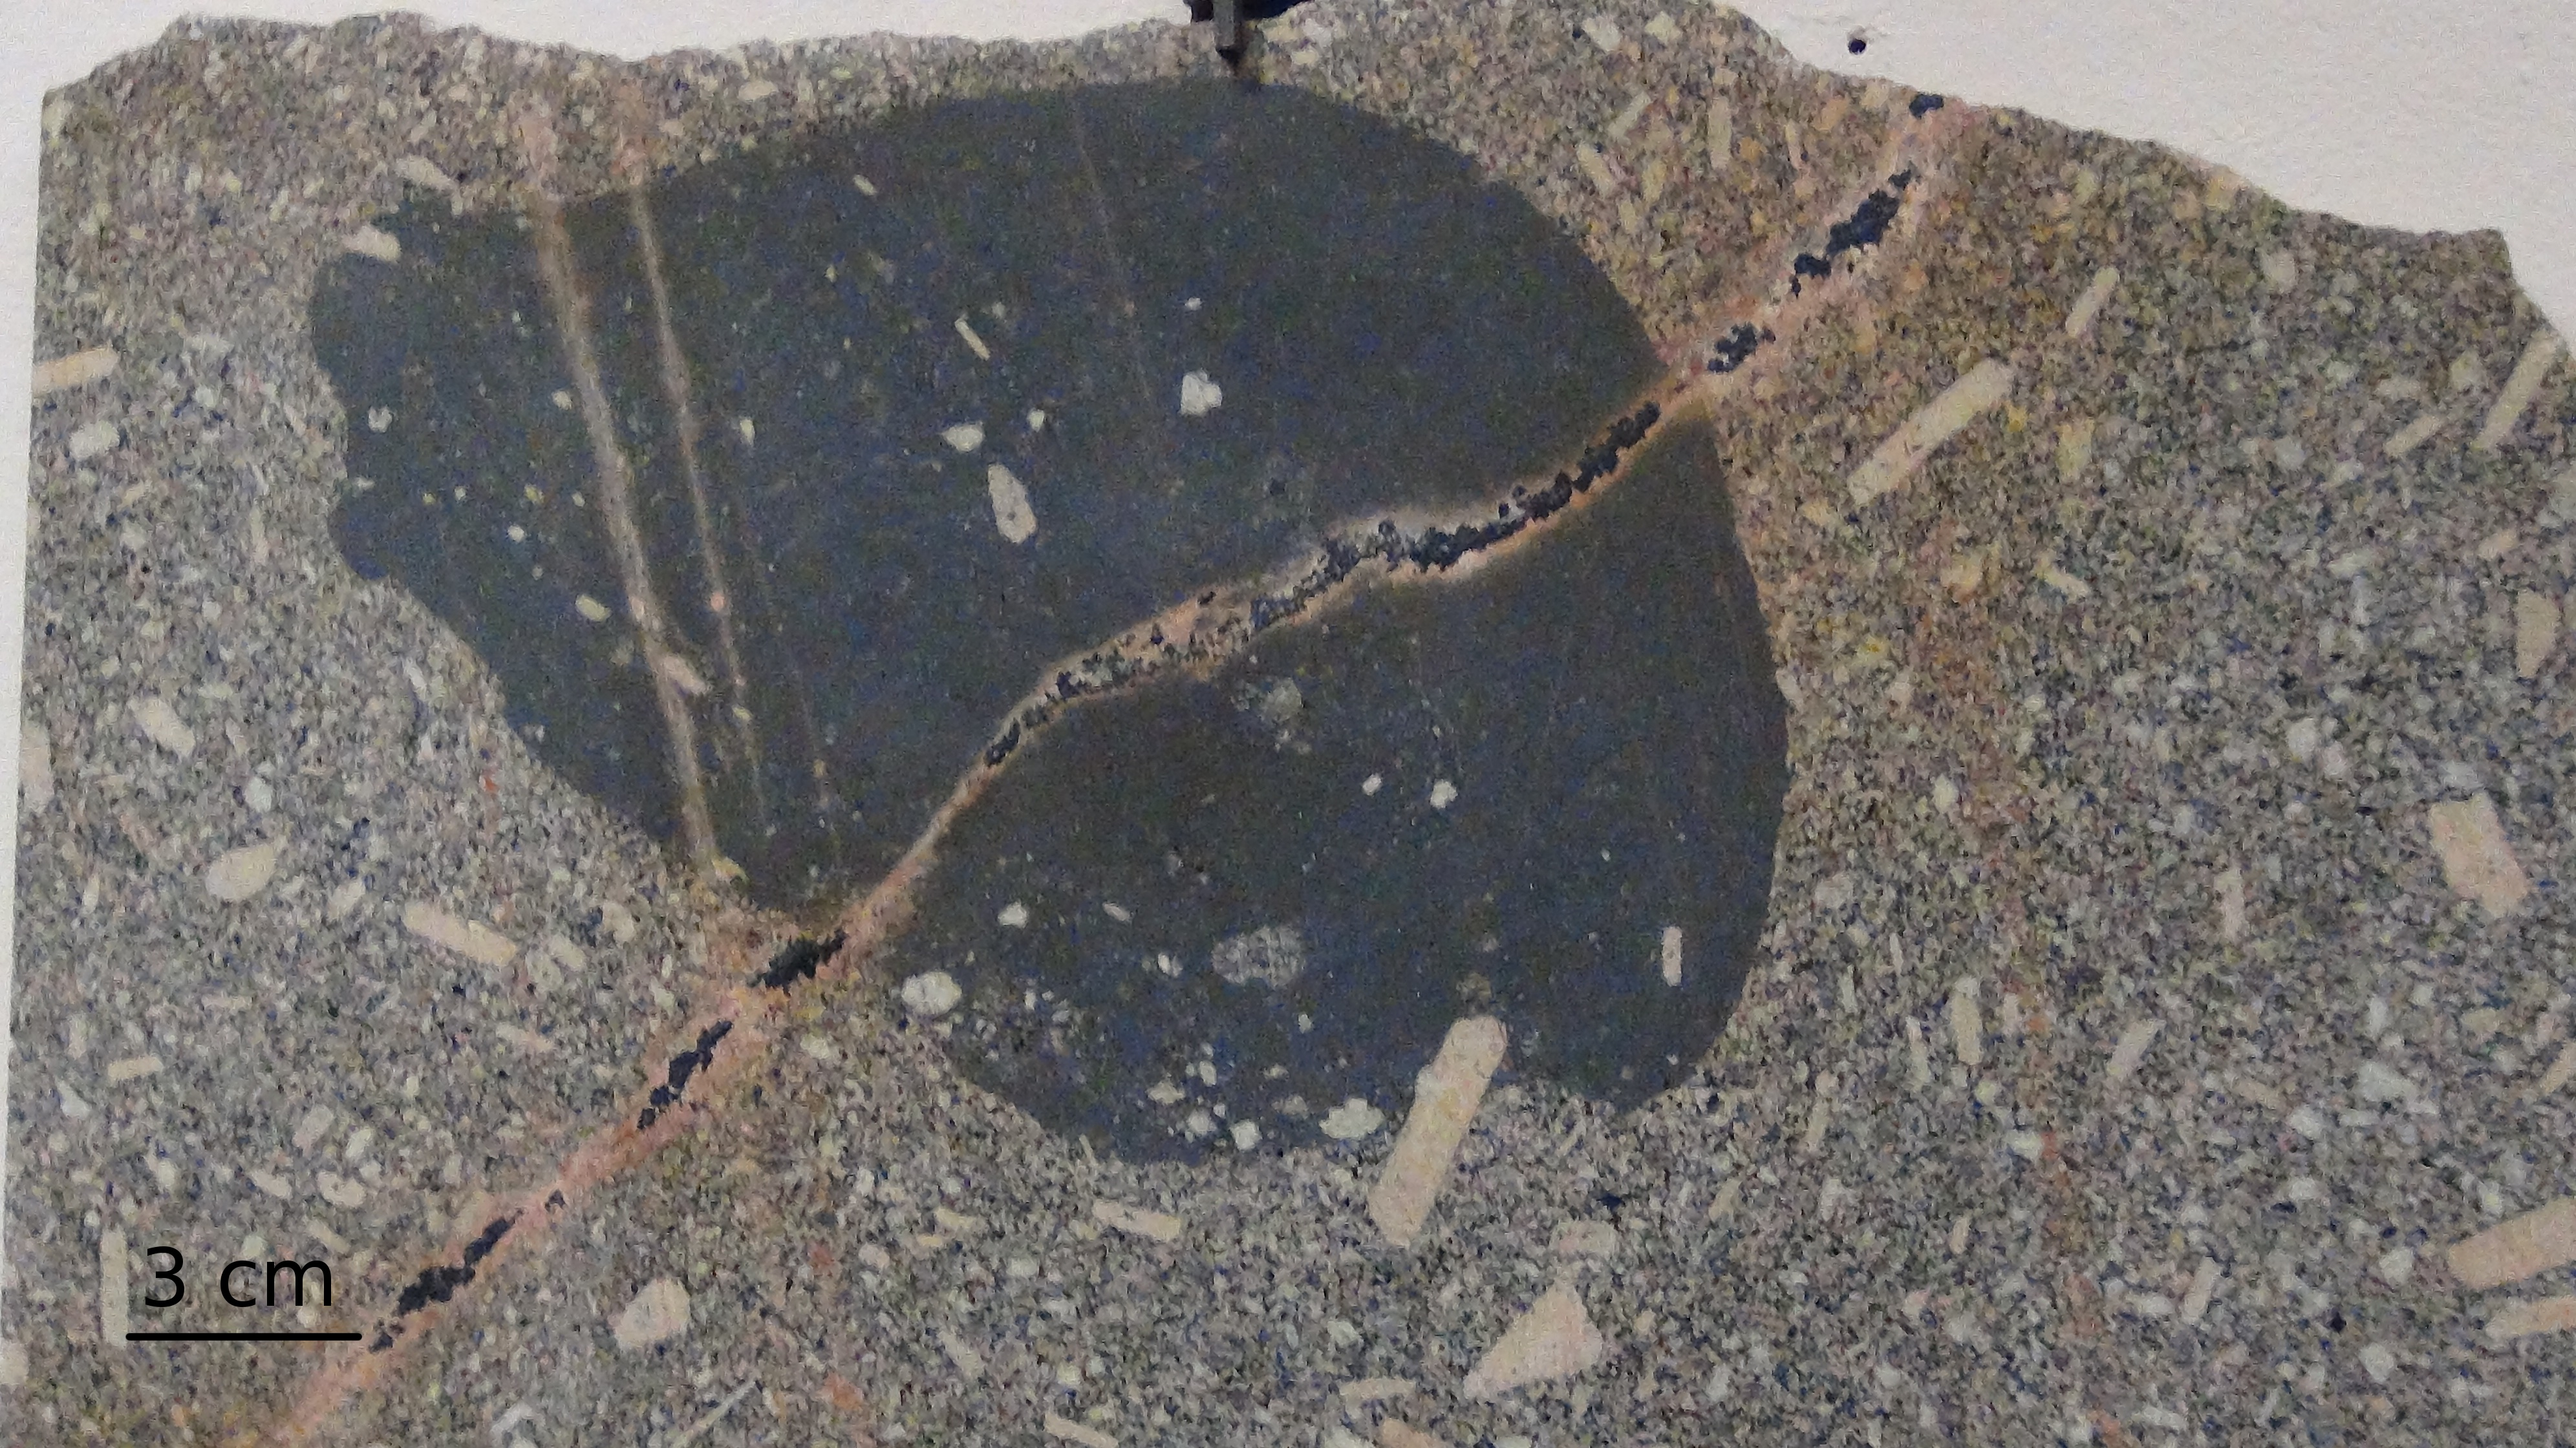
\includegraphics[width=0.4\paperwidth]{xenocryst.JPG}$$
        \end{figure}

        \vspace{-1.5cm}

        \begin{figure}
          $$\includegraphics[width=0.4\paperwidth]{UN1C_plg1.png}$$
        \end{figure}

      \end{column}

      \begin{column}{0.5\paperwidth}

        \vspace{-2cm}

        \begin{figure}
          $$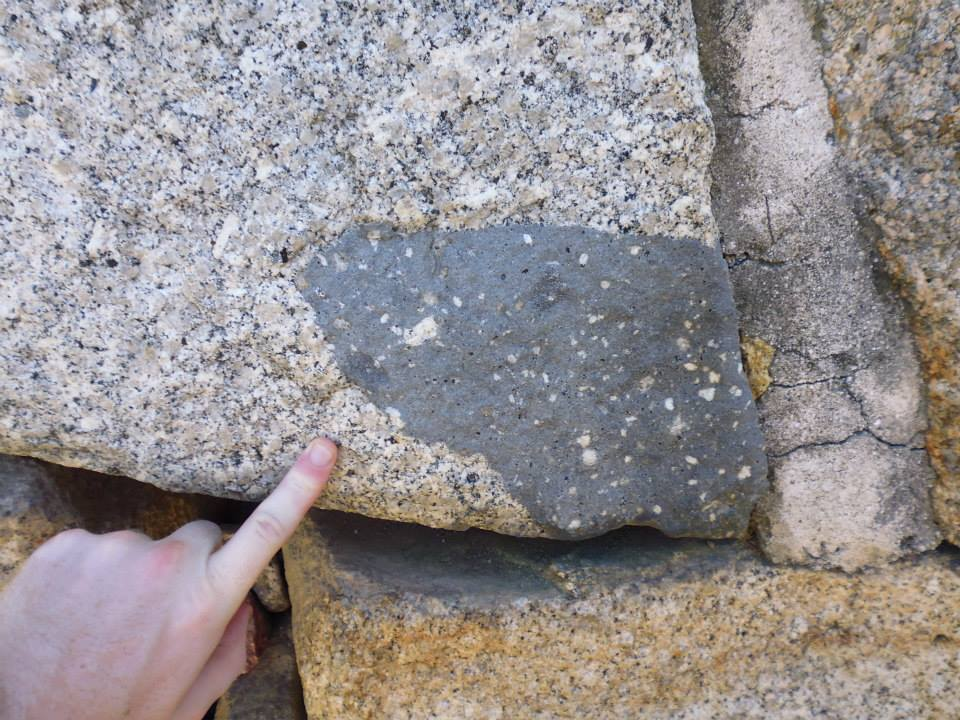
\includegraphics[width=0.4\paperwidth]{Hiroshima_castle.jpg}$$
        \end{figure}

        \vspace{-1.5cm}

        \begin{figure}
          $$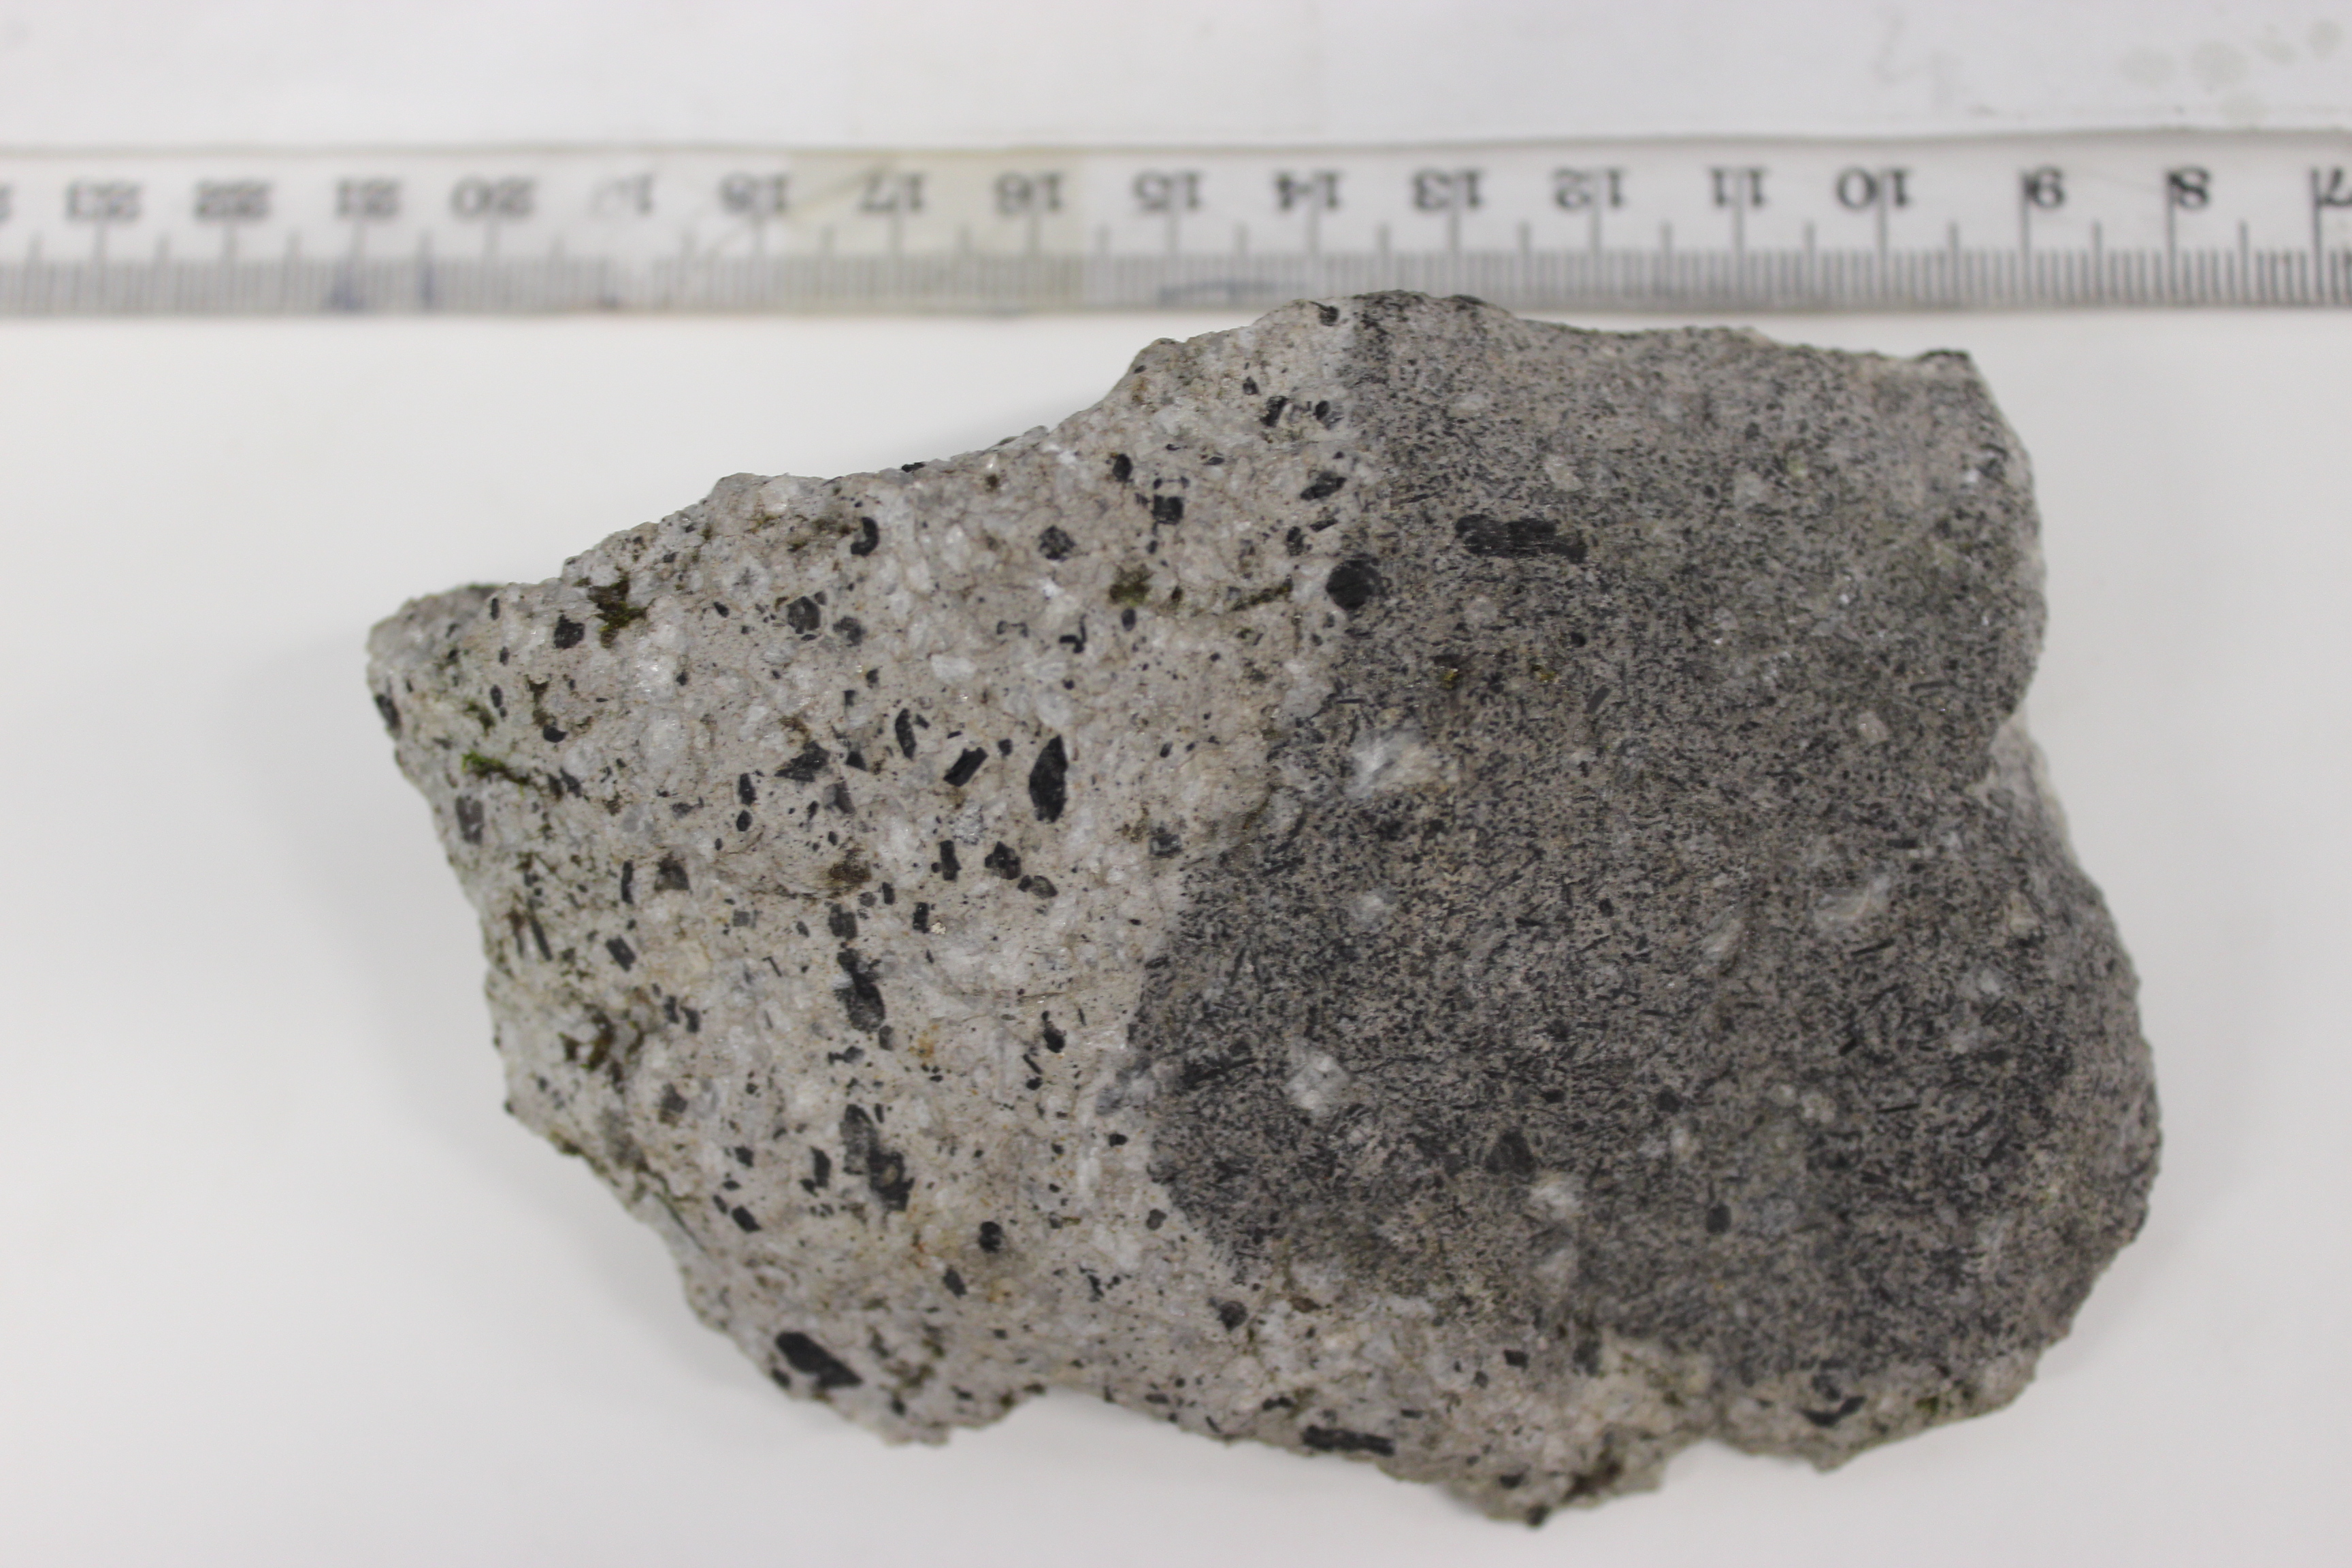
\includegraphics[width=0.4\paperwidth]{un1(c).JPG}$$
        \end{figure}

      \end{column}

    \end{columns}


  \end{center}
\end{frame}

%-----------------------------------------------

\begin{frame}
  \frametitle{Implications of xenocrysts}

  \begin{columns}[t]

    \begin{column}{0.5\paperwidth}

      \vspace{-1.7cm}
      
      \begin{figure}
        $$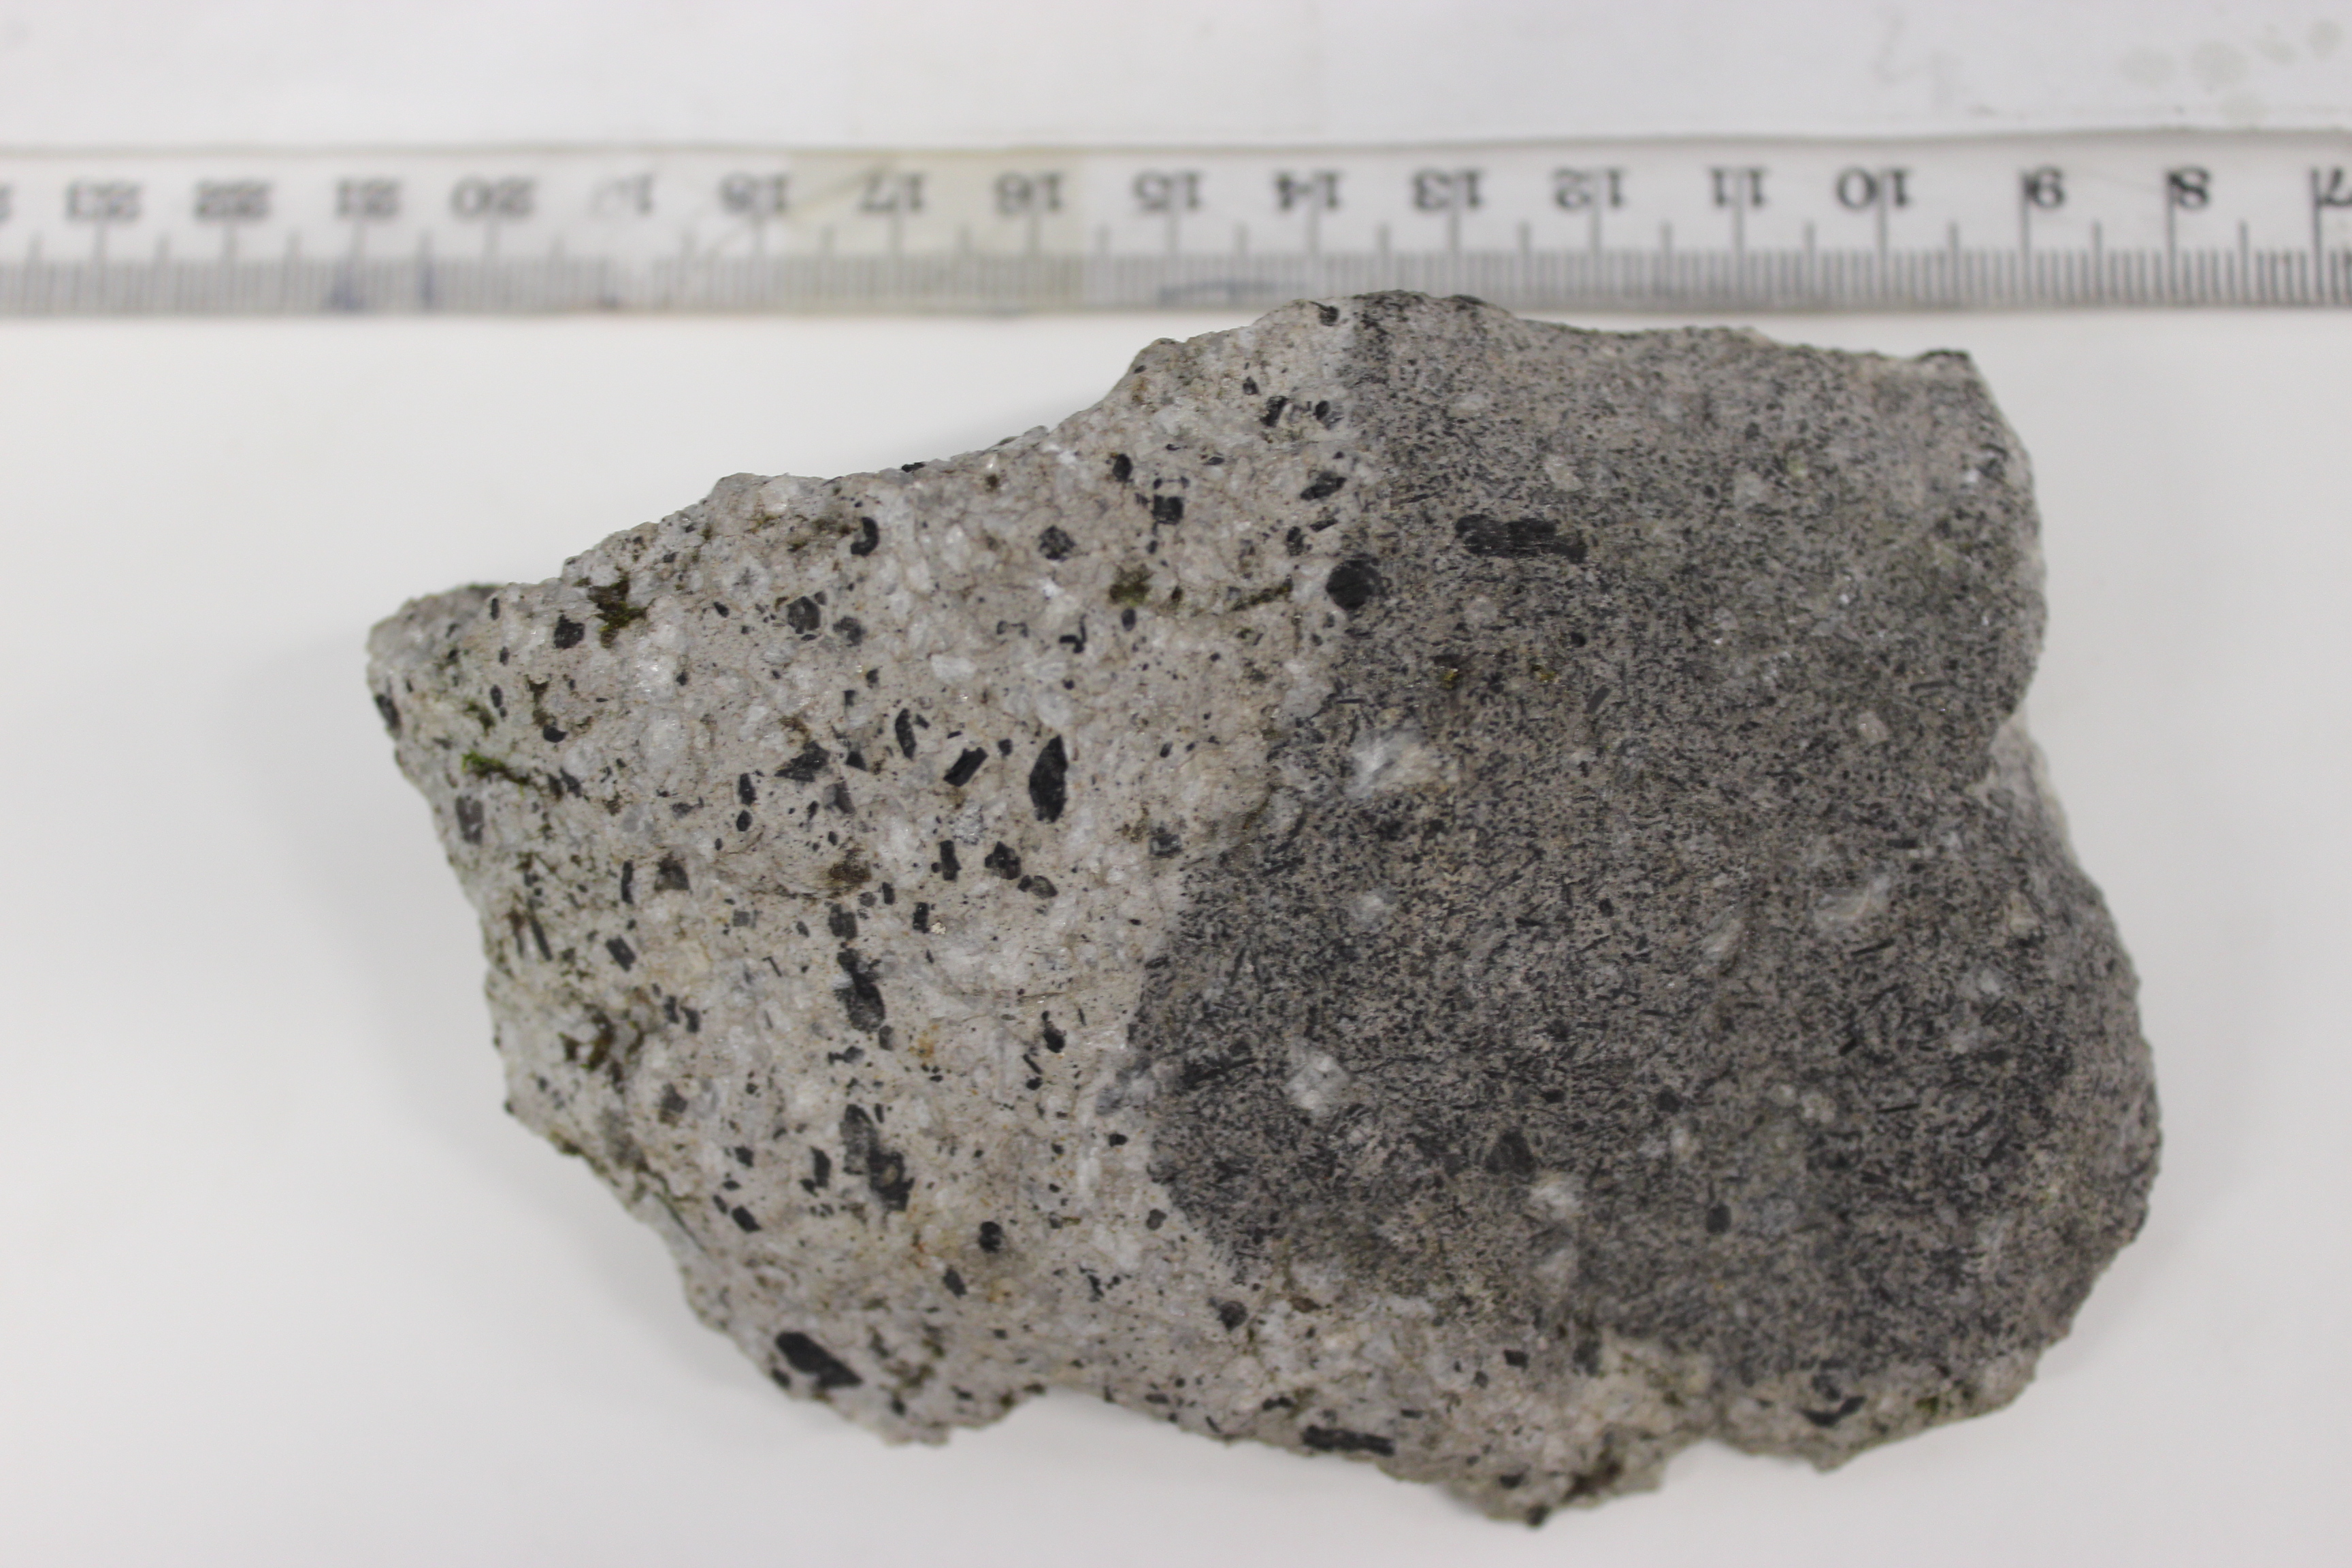
\includegraphics[width=0.4\paperwidth]{un1(c).JPG}$$
      \end{figure}
%      \vspace{-0.8cm}
      \centering

      \small Thermal models $\implies$ equilibration $\approx$ 1 hour \tiny(Jaeger 1968) \\
      \vspace{0.5cm}
      \small Experiments $\implies$ resorption zones require 0.3 - 8 days to form \tiny(Nakamura and Shimakita 1998)\\
      \vspace{0.5cm}
      \small Crystals encorporated prior to enclave formation \tiny (Browne et al. 2006)
    \end{column}

    \begin{column}{0.5\paperwidth}
      \centering
      \small Mt Unzen - Porphyritic enclaves with hornblende and plagioclase xenocrysts 
      \vspace{-1cm}
      \begin{figure}
        $$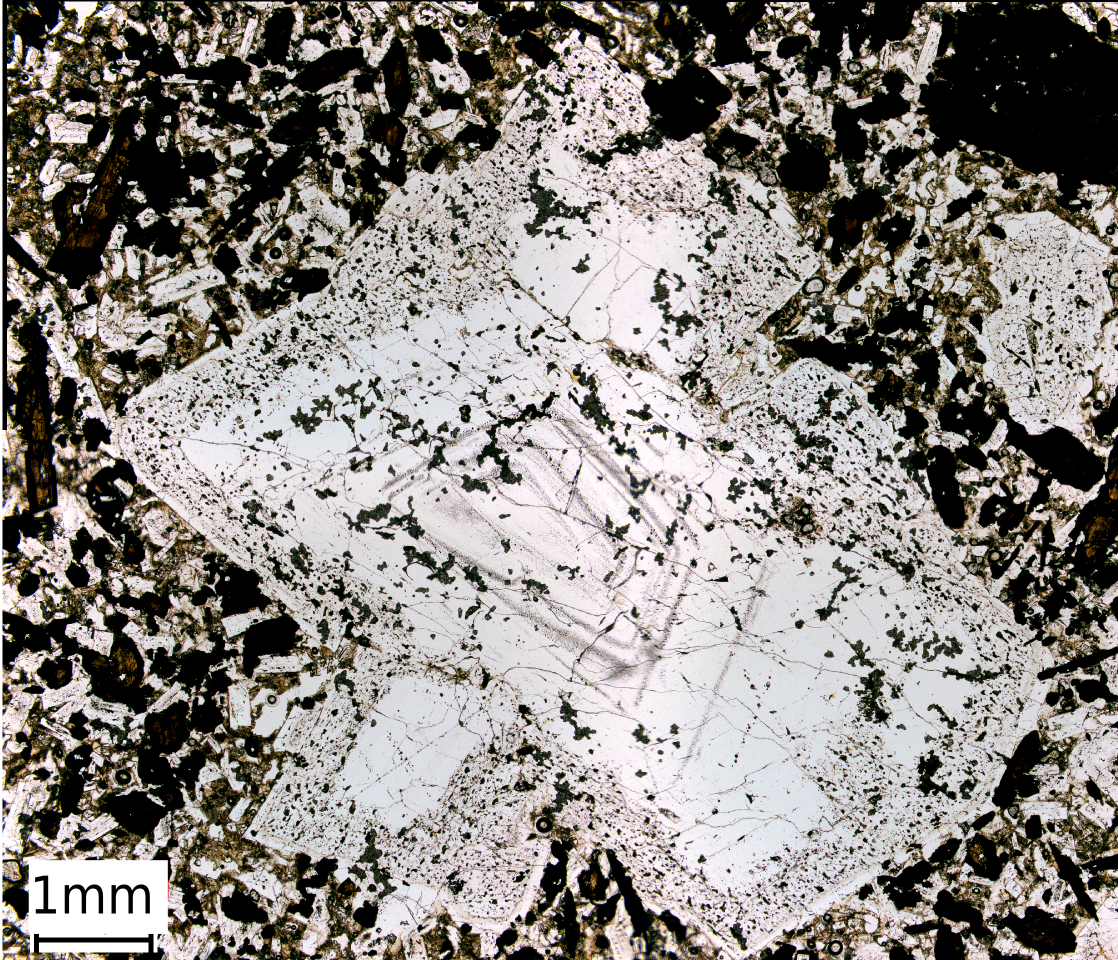
\includegraphics[width=0.4\paperwidth]{resorbed_xeno.png}$$
      \end{figure}

      \vspace{-2.3cm}

      \begin{columns}[t]
        \begin{column}{0.2\paperwidth}
          \begin{figure}
            $$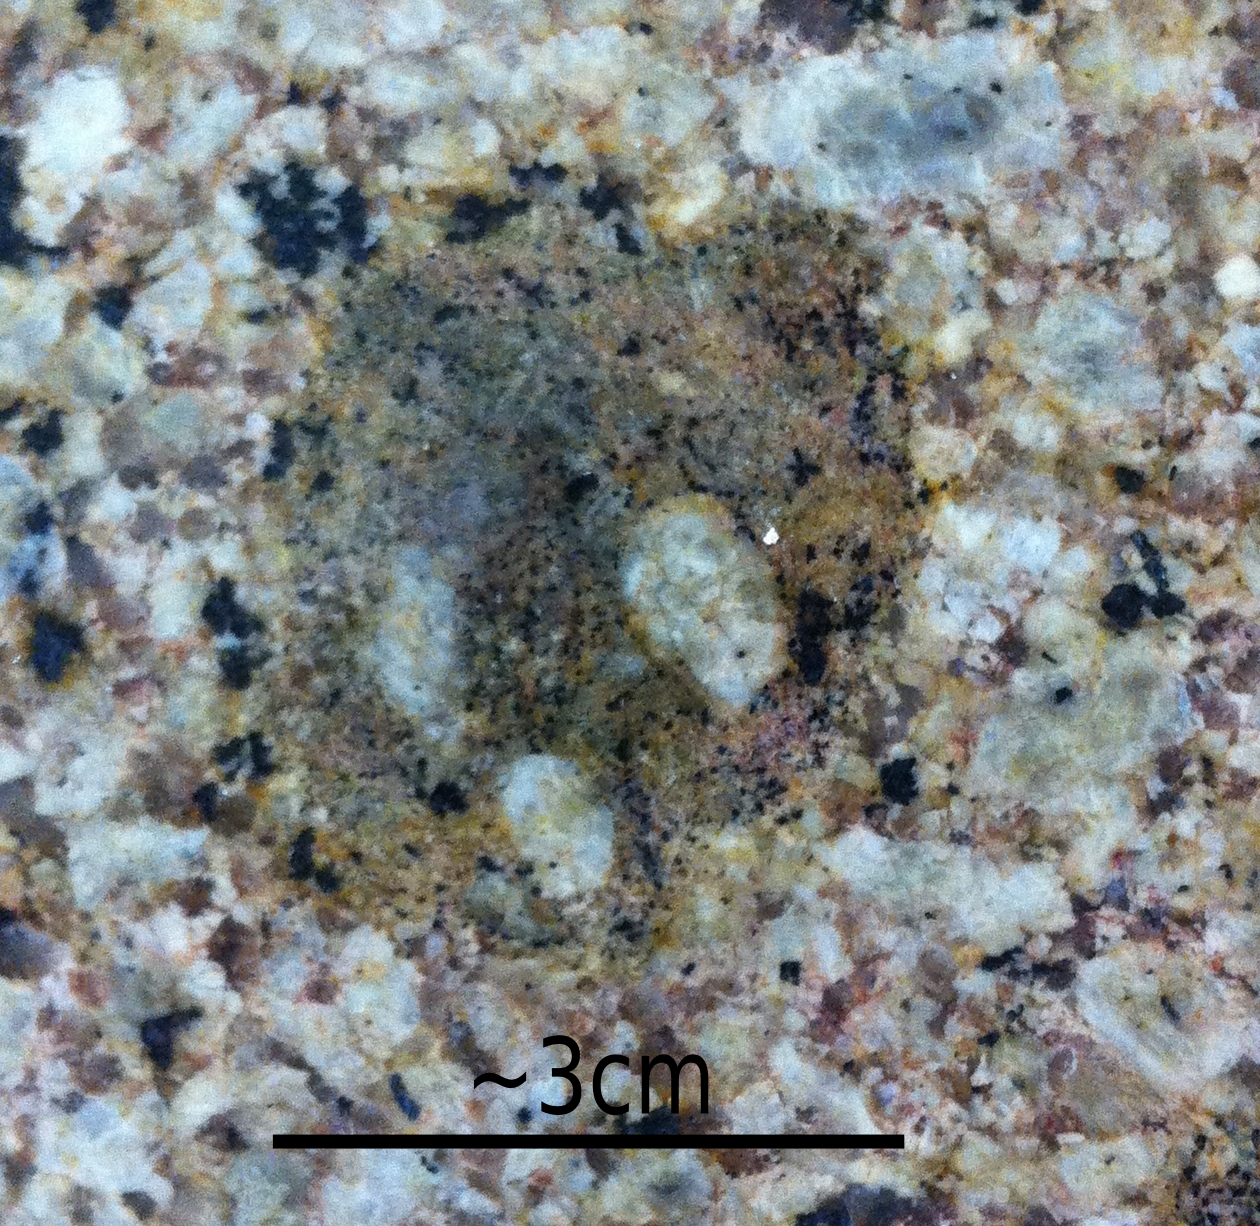
\includegraphics[width=0.2\paperwidth]{austin.png}$$
          \end{figure}
        \end{column}

        \begin{column}{0.2\paperwidth}
          \vspace{2cm}

          Even smaller enclaves contain xenocrysts
        \end{column}

      \end{columns}
    \end{column}
  \end{columns}
\end{frame}

%-----------------------------------------------

\begin{frame}{Gravitational Settling}
  \begin{columns}[t]
 
    \begin{column}{0.5\paperwidth}
      \centering

      \vspace{-1cm}

      \begin{figure}
        $$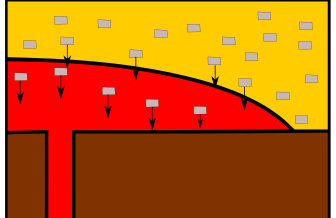
\includegraphics[width=\textwidth]{grav_settle.png}$$
      \end{figure}

      \vspace{-2.4cm}

      \begin{columns}[t]

        \begin{column}{0.5\textwidth}

          \begin{figure}
            $$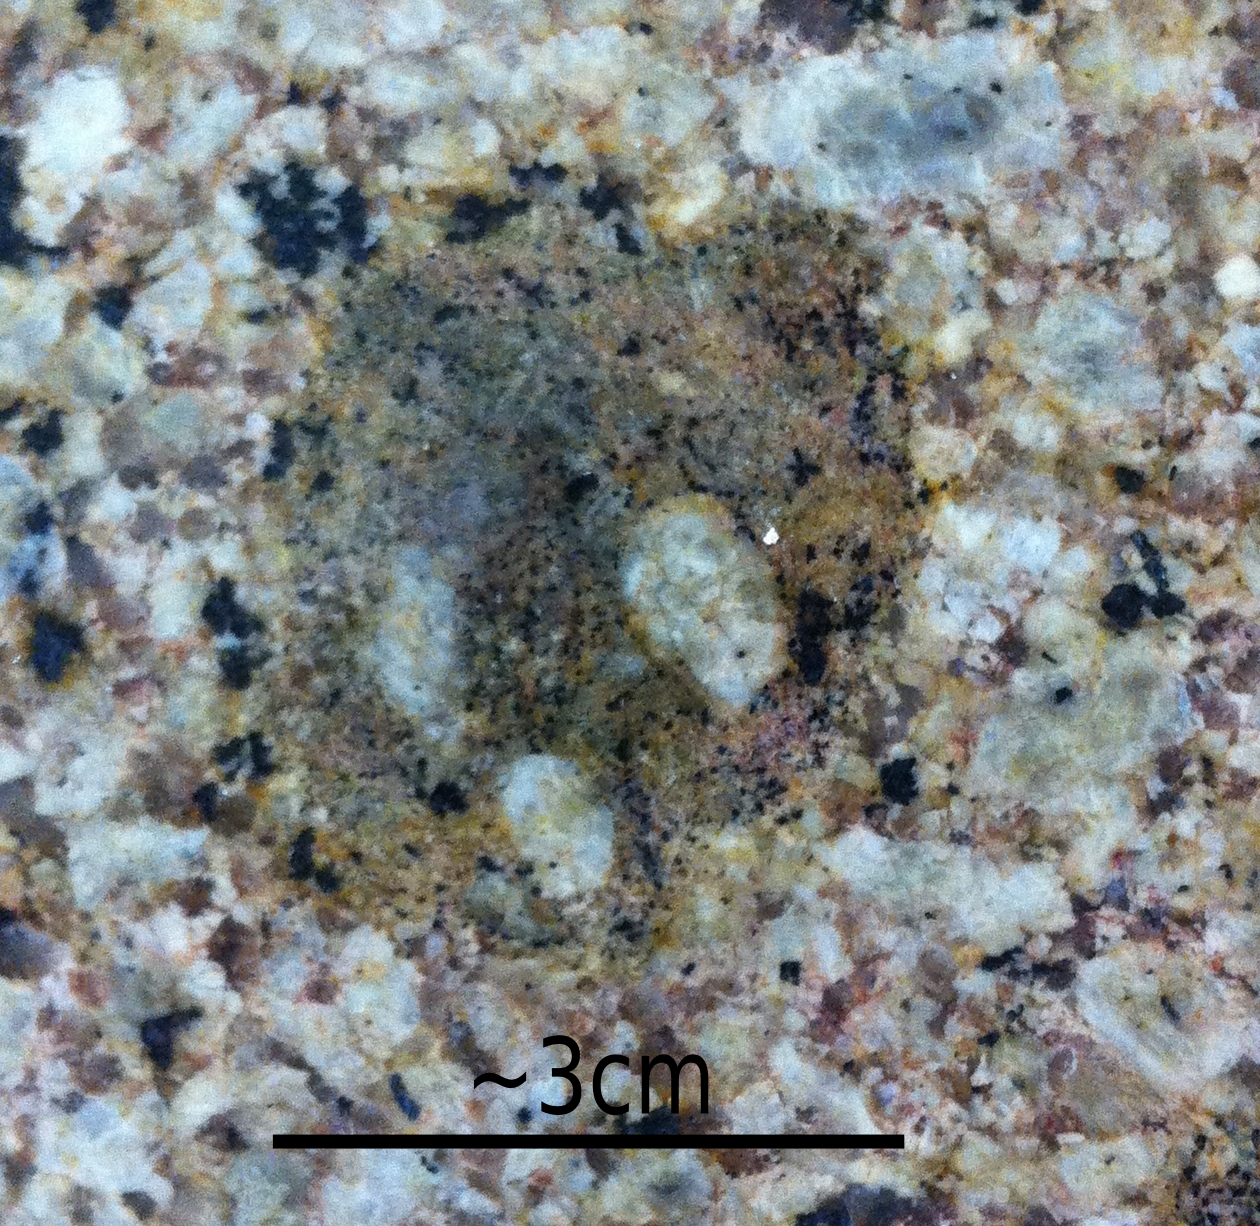
\includegraphics[width=0.8\textwidth]{austin.png}$$
          \end{figure}

          \vspace{-0.7cm}

          \centering \tiny Credit Jon Blundy

        \end{column}

        \begin{column}{0.5\textwidth}

          \begin{figure}
            $$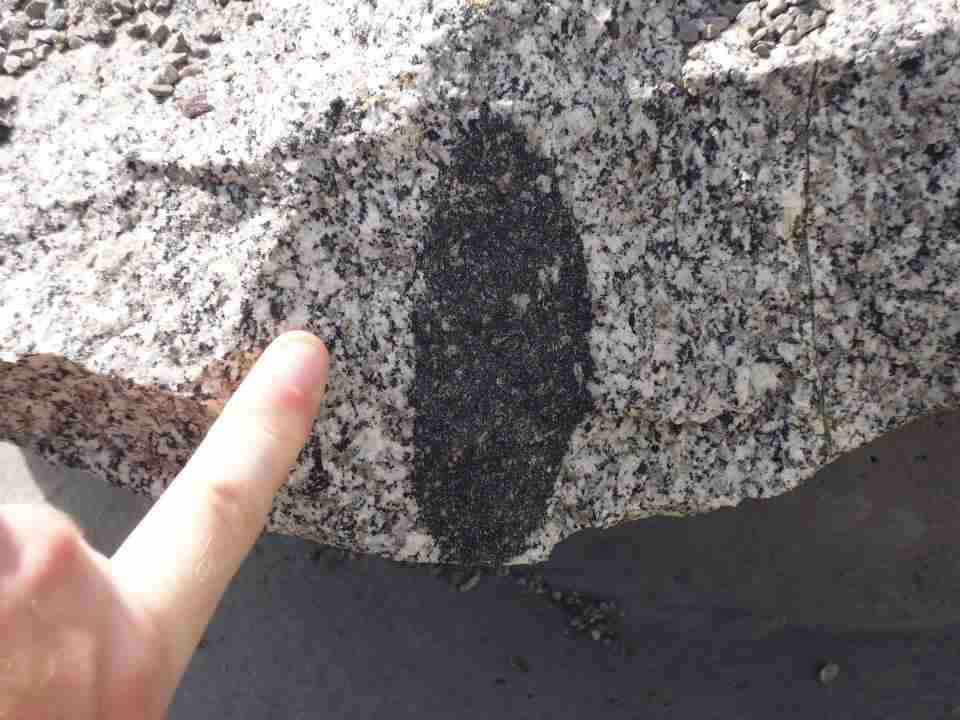
\includegraphics[width=0.9\textwidth]{Moscow_statue.jpg}$$
          \end{figure}

        \end{column}

      \end{columns}

    \end{column}

    \begin{column}{0.5\paperwidth}
      \vspace{-1.5cm}
      \begin{figure}
        $$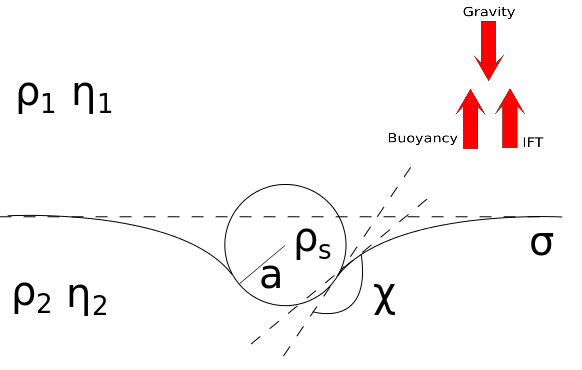
\includegraphics[width=0.4\paperwidth]{physical_formulation(2).png}$$
      \end{figure}
      \vspace{-1cm}
      \begin{itemize}
        \item $\rho_{1(2)} =$ Density of fluid 1(2)
        \item $\eta_{1(2)} =$ Viscosity of fluid 1(2)
        \item $\sigma =$ Interfacial tension (IFT)
        \item $a =$ Radius
        \item $\rho_{s} =$ Particle density
        \item $\chi =$ Contact angle
      \end{itemize}

    \end{column}
  \end{columns}
\end{frame}

%-----------------------------------------------

\begin{frame}
  \frametitle{Questions}

  \begin{itemize}
    \item For what conditions is sinking assciated with entrainment of upper phase fluid? \\
      ~ Consequences for magma hybridisation
       \vspace{0.5cm}
    \item What is the timescale of sinking? \\
      ~ Important if other timescales matter e.g. solidifcation
      \vspace{1cm}
  \end{itemize}

  \vspace{-2.5cm}

  \begin{columns}[t]

    \begin{column}{0.5\paperwidth}

      \begin{figure}
        $$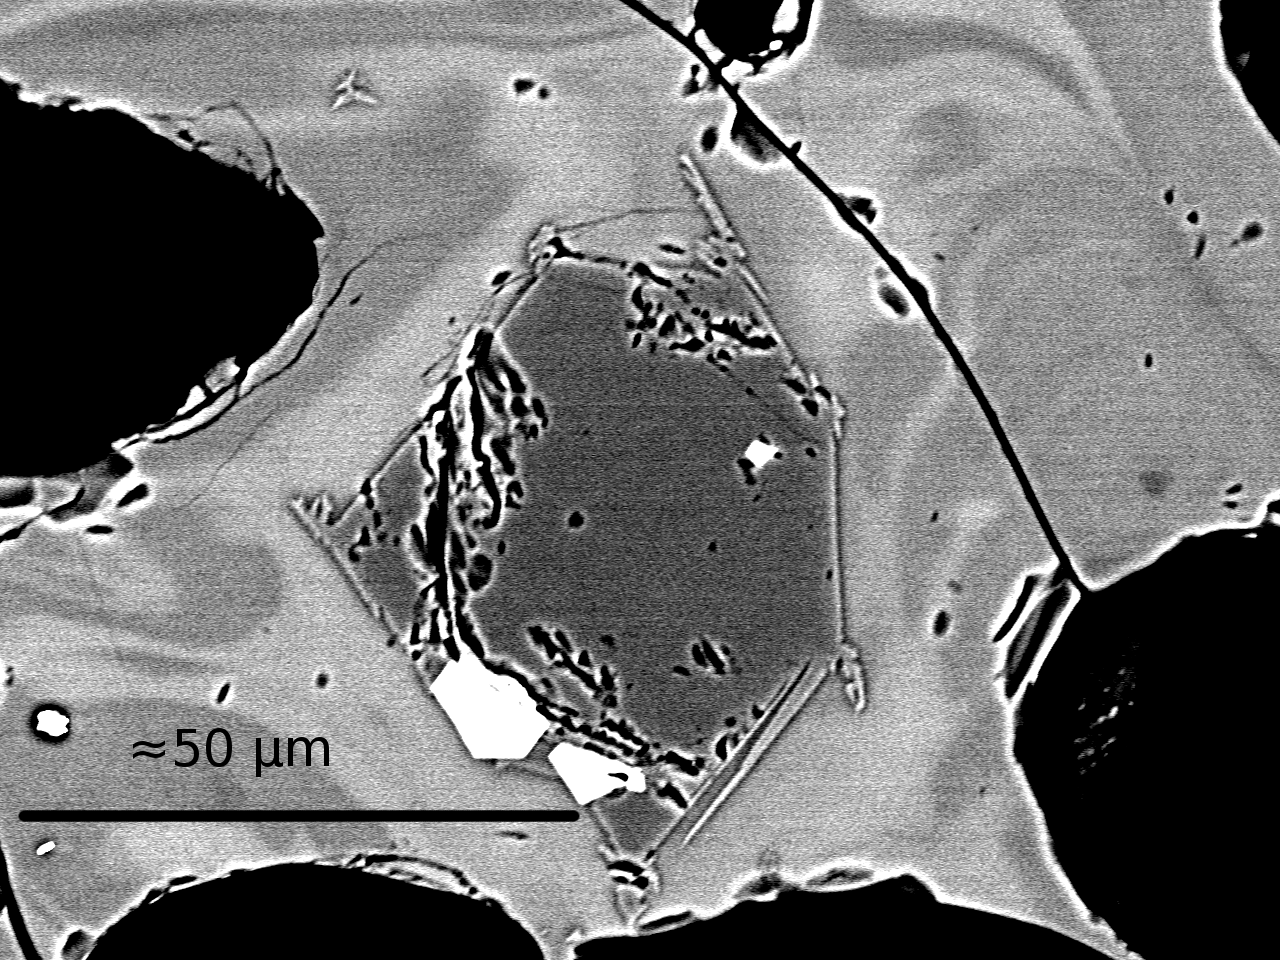
\includegraphics[width=0.9\textwidth]{olivine_xeno.png}$$
      \end{figure}

      \vspace{-0.7cm}

      \centering      \tiny Credit: Geoff Kilgour
    \end{column}

    \begin{column}{0.5\paperwidth}

      \begin{figure}
        $$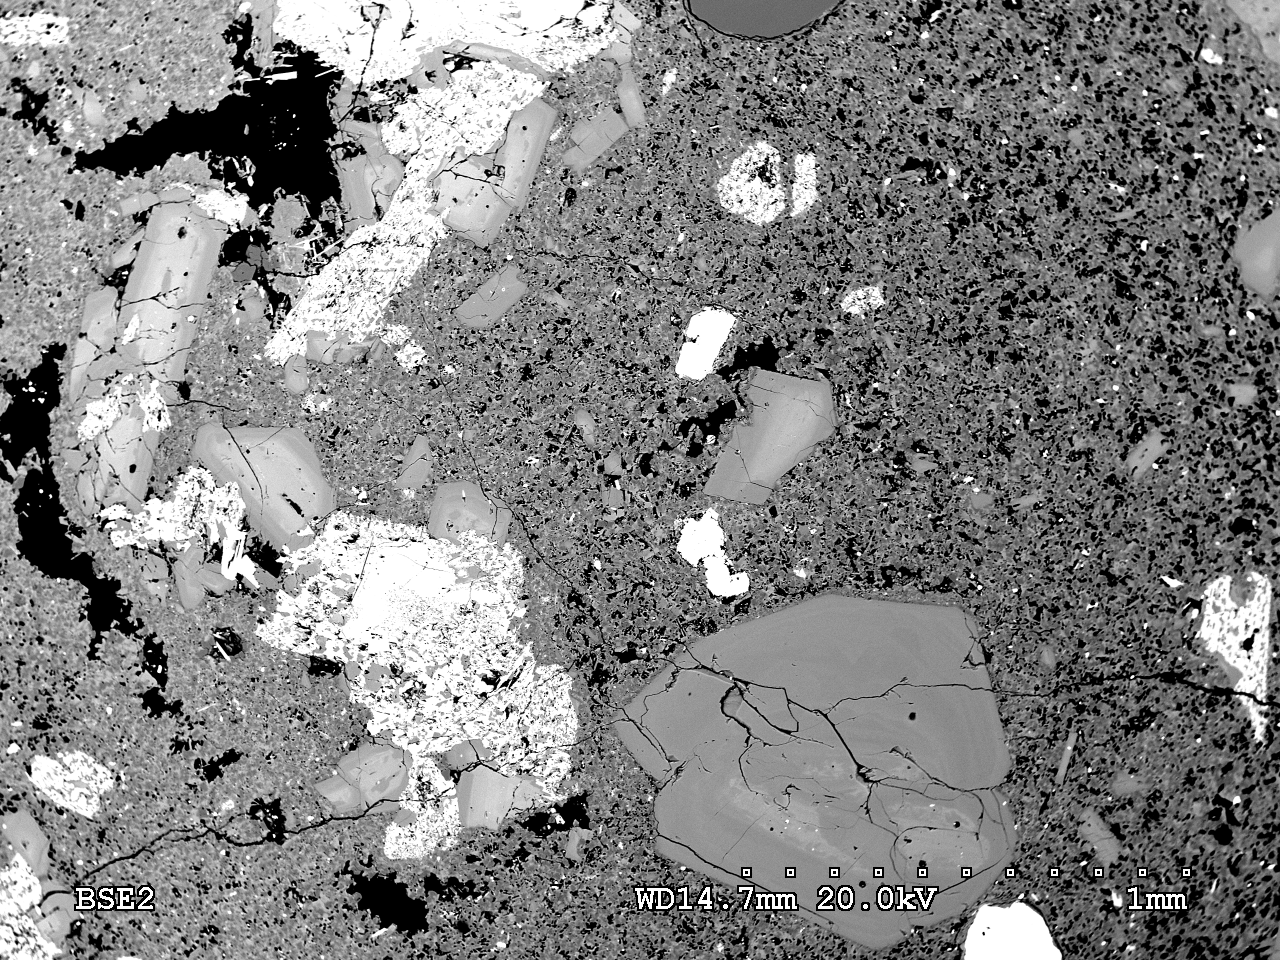
\includegraphics[width=0.9\textwidth]{grd_var_bse.png}$$
      \end{figure}

    \end{column}

  \end{columns}
\end{frame}


%----------------------------------------------

\begin{frame}{Dimensionless Parameters}

  \begin{figure}
    $$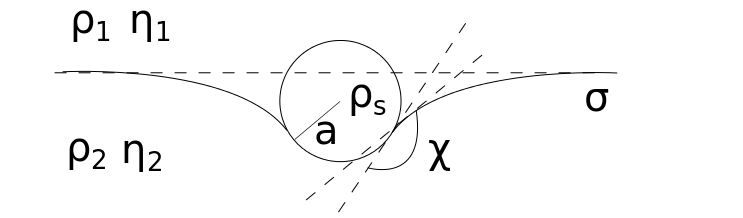
\includegraphics[width=0.9\paperwidth]{physical_formulation.png}$$
  \end{figure}

  \begin{columns}[c]
    \begin{column}{0.3\paperwidth}
      \centering
      Bond Number
      \begin{equation}
        \Bo = \frac{(\rho_{2} - \rho_{1}) g a^{2}}{\sigma} \nonumber
      \end{equation}
    \end{column}

    \begin{column}{0.3\paperwidth}
      \centering
      Modified Density Ratio
      \begin{equation}
        D = \frac{\rho_{s} - \rho_{1}}{\rho_{2} - \rho_{1}} \nonumber
      \end{equation}
    \end{column}

    \begin{column}{0.3\paperwidth}
      \centering
      Viscosity Ratio
      \begin{equation}
        \lambda = \frac{\eta_{2}}{\eta_{1}} \nonumber
      \end{equation}
    \end{column}

  \end{columns}

\end{frame}

%-----------------------------------------------
\begin{frame}
  \frametitle{Length- and time-scales}

  \begin{columns}

    \begin{column}{0.5\paperwidth}
      \centering

      Capillary length 

      \begin{equation}
        l_{\text{c}} = \left(\frac{\sigma}{(\rho_{2} - \rho_{1}) g}\right)^{1/2} \nonumber
      \end{equation}

      \vspace{1cm}

      For $a < l_{\text{c}}$, $\Bo < 1$, expect $\sigma$ to control the interfacial response

      \vspace{1cm}

      For $a < l_{\text{c}}$, $\Bo > 1$, expect density contrast to control the interfacial response

    \end{column}

    \begin{column}{0.5\paperwidth}
      \centering

      Multiple possible timescales e.g.

      \begin{equation}
        t = \frac{\eta_{n} l_{\text{c}}}{\sigma}, \quad t = \frac{\eta_{n}}{(\rho_{\text{s}} - \rho_{n}) g a}, \nonumber
      \end{equation}

      $n = 1,2$

      \vspace{1cm}

      Choose to non-dimensionalise with

      \begin{equation}
        t_{\text{i}} = \frac{\eta_{1} a}{\sigma} \nonumber
      \end{equation}
    \end{column}

  \end{columns}

\end{frame}

%-----------------------------------------------

\begin{frame}
  \frametitle{Experiments}

  \begin{columns}

    \begin{column}{0.5\paperwidth}
      \vspace{-1cm}

      \begin{figure}
        $$\includegraphics[width=0.5\paperwidth]{tank_labelled.png}$$
      \end{figure}

    \end{column}

    \begin{column}{0.5\paperwidth}
      \centering

      Glass spheres of various radii 2-10 mm \\

      \vspace{0.5cm}

      Water content in syrup from 0-5\% \\

      \vspace{0.5cm}

      Grade of PDMS oil \\

      \vspace{0.5cm}

      Temperature from 0-32$^{\circ}$C \\

      \vspace{1cm}

      Can achieve ranges: \\

      \vspace{0.5cm}

      $0.1 \leq \Bo \leq 5$ \\

      \vspace{0.5cm}

      $10^{-2} \leq \lambda \leq 10^{3}$ \\
 
      \vspace{0.5cm}

      $D \approx 3.3$ \\
    \end{column}

  \end{columns}
\end{frame}

%-----------------------------------------------

\begin{frame}
  \frametitle{Modes of Transfer}

  \begin{columns}
    \begin{column}{0.7\paperwidth}
      \centering 
      Tailing Mode
      \vspace{-0.9cm}
      \begin{figure}
        $$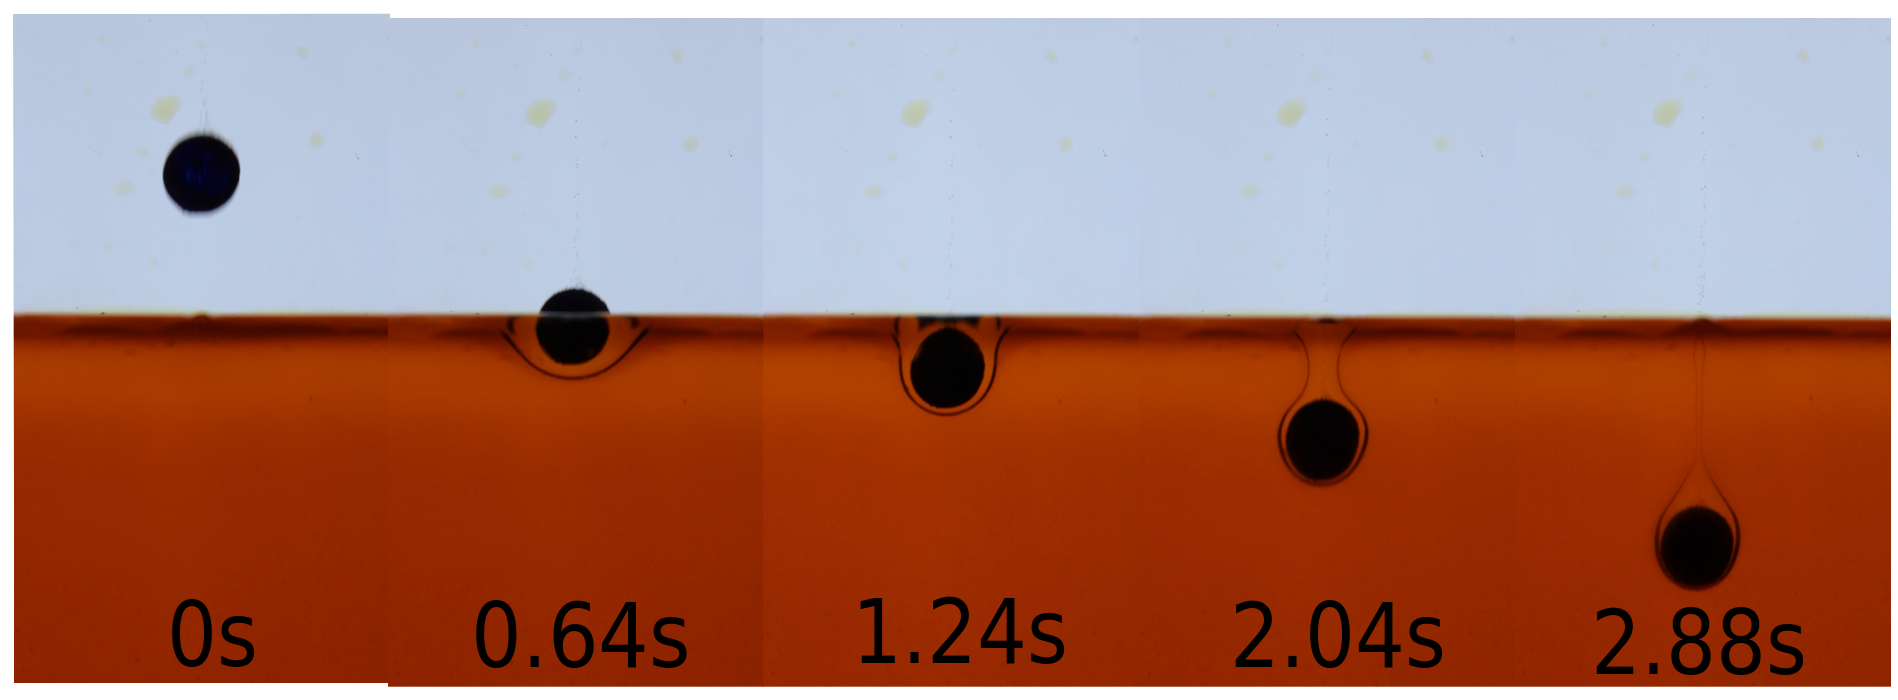
\includegraphics[width=0.7\paperwidth]{D24.png}$$
      \end{figure}
      \vspace{-0.8cm}
      Film Drainage Mode
      \vspace{-0.9cm}
      \begin{figure}
        $$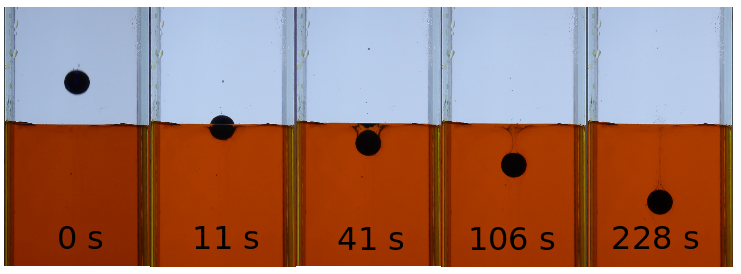
\includegraphics[width=0.7\paperwidth]{F42.png}$$
      \end{figure}
    \end{column}

    \begin{column}{0.3\paperwidth}

       $ \Bo = 2.39 \pm 0.2$

       \vspace{0.5cm}

       $ D = 3.4777 \pm 0.007$

       \vspace{0.5cm}

       $ \lambda = 3.9 \pm 0.4$

       \vspace{2cm}

       $ \Bo = 4.0 \pm 0.1$

       \vspace{0.5cm}

       $ D = 3.248 \pm 0.005$

       \vspace{0.5cm}

       $ \lambda = 259 \pm 6$
    \end{column}
\end{columns}
\end{frame}

%-----------------------------------------------

\begin{frame}
\frametitle{The Tailing Mode}

\centering
$\Bo = 4.30 \pm 0.05 \quad \quad D = 3.22 \pm 0.01 \quad \quad \lambda = 1.65 \pm 0.06$

  \begin{figure}
    $$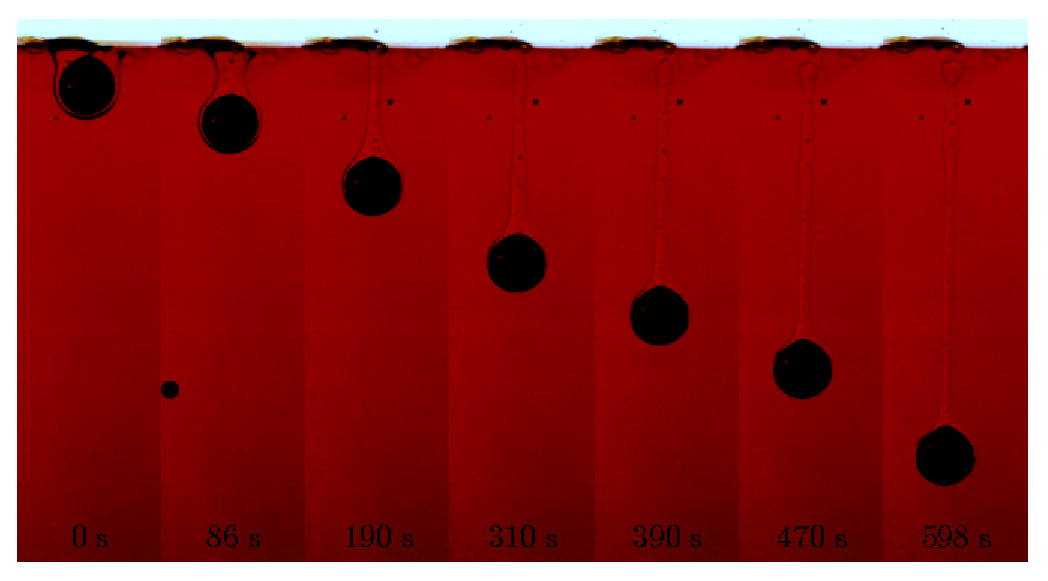
\includegraphics[width=\textwidth]{tail_detail.eps}$$
  \end{figure}


\end{frame}
%----------------------------------------------

\begin{frame}
  \frametitle{Modes of Transfer}

  \vspace{-1cm}

\begin{figure}
  \begin{center}
    \resizebox{\textwidth}{!}{% GNUPLOT: LaTeX picture with Postscript
\begingroup
  \makeatletter
  \providecommand\color[2][]{%
    \GenericError{(gnuplot) \space\space\space\@spaces}{%
      Package color not loaded in conjunction with
      terminal option `colourtext'%
    }{See the gnuplot documentation for explanation.%
    }{Either use 'blacktext' in gnuplot or load the package
      color.sty in LaTeX.}%
    \renewcommand\color[2][]{}%
  }%
  \providecommand\includegraphics[2][]{%
    \GenericError{(gnuplot) \space\space\space\@spaces}{%
      Package graphicx or graphics not loaded%
    }{See the gnuplot documentation for explanation.%
    }{The gnuplot epslatex terminal needs graphicx.sty or graphics.sty.}%
    \renewcommand\includegraphics[2][]{}%
  }%
  \providecommand\rotatebox[2]{#2}%
  \@ifundefined{ifGPcolor}{%
    \newif\ifGPcolor
    \GPcolorfalse
  }{}%
  \@ifundefined{ifGPblacktext}{%
    \newif\ifGPblacktext
    \GPblacktexttrue
  }{}%
  % define a \g@addto@macro without @ in the name:
  \let\gplgaddtomacro\g@addto@macro
  % define empty templates for all commands taking text:
  \gdef\gplbacktext{}%
  \gdef\gplfronttext{}%
  \makeatother
  \ifGPblacktext
    % no textcolor at all
    \def\colorrgb#1{}%
    \def\colorgray#1{}%
  \else
    % gray or color?
    \ifGPcolor
      \def\colorrgb#1{\color[rgb]{#1}}%
      \def\colorgray#1{\color[gray]{#1}}%
      \expandafter\def\csname LTw\endcsname{\color{white}}%
      \expandafter\def\csname LTb\endcsname{\color{black}}%
      \expandafter\def\csname LTa\endcsname{\color{black}}%
      \expandafter\def\csname LT0\endcsname{\color[rgb]{1,0,0}}%
      \expandafter\def\csname LT1\endcsname{\color[rgb]{0,1,0}}%
      \expandafter\def\csname LT2\endcsname{\color[rgb]{0,0,1}}%
      \expandafter\def\csname LT3\endcsname{\color[rgb]{1,0,1}}%
      \expandafter\def\csname LT4\endcsname{\color[rgb]{0,1,1}}%
      \expandafter\def\csname LT5\endcsname{\color[rgb]{1,1,0}}%
      \expandafter\def\csname LT6\endcsname{\color[rgb]{0,0,0}}%
      \expandafter\def\csname LT7\endcsname{\color[rgb]{1,0.3,0}}%
      \expandafter\def\csname LT8\endcsname{\color[rgb]{0.5,0.5,0.5}}%
    \else
      % gray
      \def\colorrgb#1{\color{black}}%
      \def\colorgray#1{\color[gray]{#1}}%
      \expandafter\def\csname LTw\endcsname{\color{white}}%
      \expandafter\def\csname LTb\endcsname{\color{black}}%
      \expandafter\def\csname LTa\endcsname{\color{black}}%
      \expandafter\def\csname LT0\endcsname{\color{black}}%
      \expandafter\def\csname LT1\endcsname{\color{black}}%
      \expandafter\def\csname LT2\endcsname{\color{black}}%
      \expandafter\def\csname LT3\endcsname{\color{black}}%
      \expandafter\def\csname LT4\endcsname{\color{black}}%
      \expandafter\def\csname LT5\endcsname{\color{black}}%
      \expandafter\def\csname LT6\endcsname{\color{black}}%
      \expandafter\def\csname LT7\endcsname{\color{black}}%
      \expandafter\def\csname LT8\endcsname{\color{black}}%
    \fi
  \fi
    \setlength{\unitlength}{0.0500bp}%
    \ifx\gptboxheight\undefined%
      \newlength{\gptboxheight}%
      \newlength{\gptboxwidth}%
      \newsavebox{\gptboxtext}%
    \fi%
    \setlength{\fboxrule}{0.5pt}%
    \setlength{\fboxsep}{1pt}%
\begin{picture}(7200.00,5040.00)%
    \gplgaddtomacro\gplbacktext{%
      \csname LTb\endcsname%
      \put(814,1144){\makebox(0,0)[r]{\strut{}$0$}}%
      \put(814,1547){\makebox(0,0)[r]{\strut{}$0.5$}}%
      \put(814,1951){\makebox(0,0)[r]{\strut{}$1$}}%
      \put(814,2354){\makebox(0,0)[r]{\strut{}$1.5$}}%
      \put(814,2758){\makebox(0,0)[r]{\strut{}$2$}}%
      \put(814,3161){\makebox(0,0)[r]{\strut{}$2.5$}}%
      \put(814,3565){\makebox(0,0)[r]{\strut{}$3$}}%
      \put(814,3968){\makebox(0,0)[r]{\strut{}$3.5$}}%
      \put(814,4372){\makebox(0,0)[r]{\strut{}$4$}}%
      \put(814,4775){\makebox(0,0)[r]{\strut{}$4.5$}}%
      \put(946,924){\makebox(0,0){\strut{}$0.01$}}%
      \put(1922,924){\makebox(0,0){\strut{}$0.1$}}%
      \put(2898,924){\makebox(0,0){\strut{}$1$}}%
      \put(3875,924){\makebox(0,0){\strut{}$10$}}%
      \put(4851,924){\makebox(0,0){\strut{}$100$}}%
      \put(5827,924){\makebox(0,0){\strut{}$1000$}}%
      \put(6803,924){\makebox(0,0){\strut{}$10000$}}%
    }%
    \gplgaddtomacro\gplfronttext{%
      \csname LTb\endcsname%
      \put(176,2959){\rotatebox{-270}{\makebox(0,0){\strut{}$\text{Bo}$}}}%
      \put(3874,594){\makebox(0,0){\strut{}$\lambda$}}%
      \csname LTb\endcsname%
      \put(3019,393){\makebox(0,0)[r]{\strut{}Film Drainage}}%
      \csname LTb\endcsname%
      \put(3019,173){\makebox(0,0)[r]{\strut{}Tailing}}%
      \csname LTb\endcsname%
      \put(5590,393){\makebox(0,0)[r]{\strut{}Float}}%
      \csname LTb\endcsname%
      \put(5590,173){\makebox(0,0)[r]{\strut{}Transitional}}%
    }%
    \gplbacktext
    \put(0,0){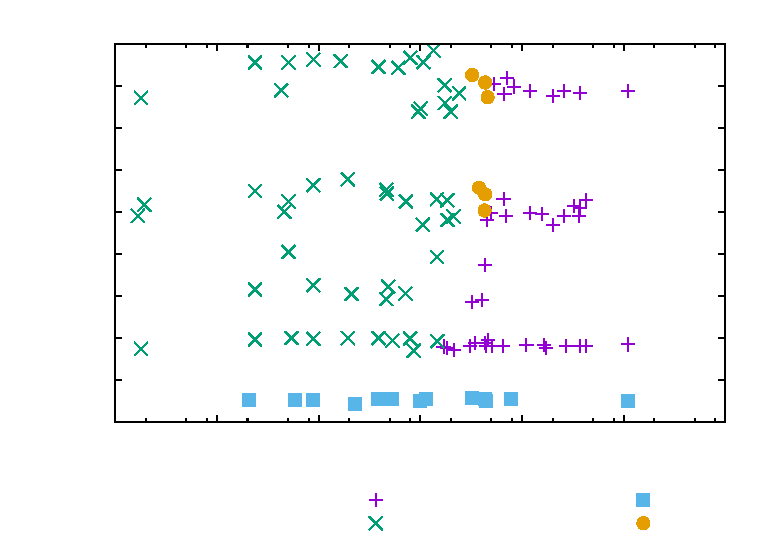
\includegraphics{low_re_bo}}%
    \gplfronttext
  \end{picture}%
\endgroup
}
  \end{center}
\end{figure}

\end{frame}
%-----------------------------------------------

\begin{frame}
  \frametitle{Sinking Timescales - Film Drainage}

  \begin{columns}[t]
    \begin{column}{0.5\paperwidth}
      \centering
      \resizebox{0.9\textwidth}{!}{% GNUPLOT: LaTeX picture with Postscript
\begingroup
  \makeatletter
  \providecommand\color[2][]{%
    \GenericError{(gnuplot) \space\space\space\@spaces}{%
      Package color not loaded in conjunction with
      terminal option `colourtext'%
    }{See the gnuplot documentation for explanation.%
    }{Either use 'blacktext' in gnuplot or load the package
      color.sty in LaTeX.}%
    \renewcommand\color[2][]{}%
  }%
  \providecommand\includegraphics[2][]{%
    \GenericError{(gnuplot) \space\space\space\@spaces}{%
      Package graphicx or graphics not loaded%
    }{See the gnuplot documentation for explanation.%
    }{The gnuplot epslatex terminal needs graphicx.sty or graphics.sty.}%
    \renewcommand\includegraphics[2][]{}%
  }%
  \providecommand\rotatebox[2]{#2}%
  \@ifundefined{ifGPcolor}{%
    \newif\ifGPcolor
    \GPcolortrue
  }{}%
  \@ifundefined{ifGPblacktext}{%
    \newif\ifGPblacktext
    \GPblacktextfalse
  }{}%
  % define a \g@addto@macro without @ in the name:
  \let\gplgaddtomacro\g@addto@macro
  % define empty templates for all commands taking text:
  \gdef\gplbacktext{}%
  \gdef\gplfronttext{}%
  \makeatother
  \ifGPblacktext
    % no textcolor at all
    \def\colorrgb#1{}%
    \def\colorgray#1{}%
  \else
    % gray or color?
    \ifGPcolor
      \def\colorrgb#1{\color[rgb]{#1}}%
      \def\colorgray#1{\color[gray]{#1}}%
      \expandafter\def\csname LTw\endcsname{\color{white}}%
      \expandafter\def\csname LTb\endcsname{\color{black}}%
      \expandafter\def\csname LTa\endcsname{\color{black}}%
      \expandafter\def\csname LT0\endcsname{\color[rgb]{1,0,0}}%
      \expandafter\def\csname LT1\endcsname{\color[rgb]{0,1,0}}%
      \expandafter\def\csname LT2\endcsname{\color[rgb]{0,0,1}}%
      \expandafter\def\csname LT3\endcsname{\color[rgb]{1,0,1}}%
      \expandafter\def\csname LT4\endcsname{\color[rgb]{0,1,1}}%
      \expandafter\def\csname LT5\endcsname{\color[rgb]{1,1,0}}%
      \expandafter\def\csname LT6\endcsname{\color[rgb]{0,0,0}}%
      \expandafter\def\csname LT7\endcsname{\color[rgb]{1,0.3,0}}%
      \expandafter\def\csname LT8\endcsname{\color[rgb]{0.5,0.5,0.5}}%
    \else
      % gray
      \def\colorrgb#1{\color{black}}%
      \def\colorgray#1{\color[gray]{#1}}%
      \expandafter\def\csname LTw\endcsname{\color{white}}%
      \expandafter\def\csname LTb\endcsname{\color{black}}%
      \expandafter\def\csname LTa\endcsname{\color{black}}%
      \expandafter\def\csname LT0\endcsname{\color{black}}%
      \expandafter\def\csname LT1\endcsname{\color{black}}%
      \expandafter\def\csname LT2\endcsname{\color{black}}%
      \expandafter\def\csname LT3\endcsname{\color{black}}%
      \expandafter\def\csname LT4\endcsname{\color{black}}%
      \expandafter\def\csname LT5\endcsname{\color{black}}%
      \expandafter\def\csname LT6\endcsname{\color{black}}%
      \expandafter\def\csname LT7\endcsname{\color{black}}%
      \expandafter\def\csname LT8\endcsname{\color{black}}%
    \fi
  \fi
    \setlength{\unitlength}{0.0500bp}%
    \ifx\gptboxheight\undefined%
      \newlength{\gptboxheight}%
      \newlength{\gptboxwidth}%
      \newsavebox{\gptboxtext}%
    \fi%
    \setlength{\fboxrule}{0.5pt}%
    \setlength{\fboxsep}{1pt}%
\begin{picture}(7200.00,5040.00)%
    \gplgaddtomacro\gplbacktext{%
      \csname LTb\endcsname%
      \put(814,1144){\makebox(0,0)[r]{\strut{}$5.5$}}%
      \put(814,1749){\makebox(0,0)[r]{\strut{}$6$}}%
      \put(814,2354){\makebox(0,0)[r]{\strut{}$6.5$}}%
      \put(814,2960){\makebox(0,0)[r]{\strut{}$7$}}%
      \put(814,3565){\makebox(0,0)[r]{\strut{}$7.5$}}%
      \put(814,4170){\makebox(0,0)[r]{\strut{}$8$}}%
      \put(814,4775){\makebox(0,0)[r]{\strut{}$8.5$}}%
      \put(946,924){\makebox(0,0){\strut{}$-0.2$}}%
      \put(1678,924){\makebox(0,0){\strut{}$0$}}%
      \put(2410,924){\makebox(0,0){\strut{}$0.2$}}%
      \put(3142,924){\makebox(0,0){\strut{}$0.4$}}%
      \put(3875,924){\makebox(0,0){\strut{}$0.6$}}%
      \put(4607,924){\makebox(0,0){\strut{}$0.8$}}%
      \put(5339,924){\makebox(0,0){\strut{}$1$}}%
      \put(6071,924){\makebox(0,0){\strut{}$1.2$}}%
      \put(6803,924){\makebox(0,0){\strut{}$1.4$}}%
      \put(3875,2052){\makebox(0,0){\strut{}\normalsize $-0.6 \pm 0.2$}}%
      \put(3875,3141){\makebox(0,0){\strut{}\normalsize $-0.87 \pm 0.08$}}%
      \put(3875,3873){\makebox(0,0){\strut{}\normalsize $-0.88 \pm 0.02$}}%
    }%
    \gplgaddtomacro\gplfronttext{%
      \csname LTb\endcsname%
      \put(176,2959){\rotatebox{-270}{\makebox(0,0){\strut{}$\ln(t / t_{i})$}}}%
      \put(3874,594){\makebox(0,0){\strut{}$\ln\text{Bo}$}}%
      \csname LTb\endcsname%
      \put(3019,393){\makebox(0,0)[r]{\strut{}$40 < \lambda < \; \, 50$}}%
      \csname LTb\endcsname%
      \put(3019,173){\makebox(0,0)[r]{\strut{}$100 < \lambda < 200$}}%
      \csname LTb\endcsname%
      \put(6118,393){\makebox(0,0)[r]{\strut{}$200 < \lambda < 300$}}%
    }%
    \gplbacktext
    \put(0,0){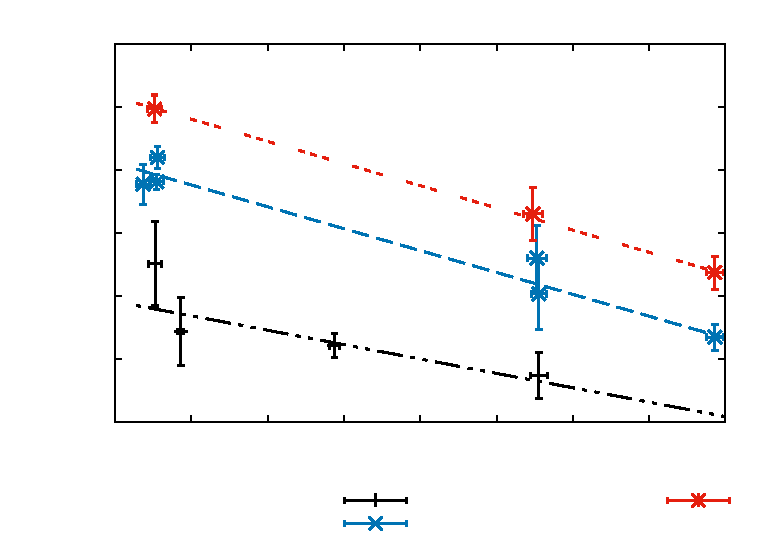
\includegraphics{out_bond_film}}%
    \gplfronttext
  \end{picture}%
\endgroup
}

\vspace{0.5cm}

$\frac{t}{t_{\text{i}}} \sim \Bo^{a} \lambda^{b}$ \\
\vspace{0.1cm}
$\ln\left(\frac{t}{t_{\text{i}}}\right) \sim a \ln\Bo + b \ln\lambda$ \\
\vspace{0.1cm}

2D fitting $\implies a = -0.80 \pm 0.05$ and $b = 0.80 \pm 0.02$ \\
\vspace{0.1cm}

$\implies  \frac{t}{t_{\text{i}}} \sim \left(\frac{\lambda}{\Bo}\right)^{4/5}$ \\
    \end{column}

    \begin{column}{0.5\paperwidth}
      \centering
      \resizebox{0.9\textwidth}{!}{% GNUPLOT: LaTeX picture with Postscript
\begingroup
  \makeatletter
  \providecommand\color[2][]{%
    \GenericError{(gnuplot) \space\space\space\@spaces}{%
      Package color not loaded in conjunction with
      terminal option `colourtext'%
    }{See the gnuplot documentation for explanation.%
    }{Either use 'blacktext' in gnuplot or load the package
      color.sty in LaTeX.}%
    \renewcommand\color[2][]{}%
  }%
  \providecommand\includegraphics[2][]{%
    \GenericError{(gnuplot) \space\space\space\@spaces}{%
      Package graphicx or graphics not loaded%
    }{See the gnuplot documentation for explanation.%
    }{The gnuplot epslatex terminal needs graphicx.sty or graphics.sty.}%
    \renewcommand\includegraphics[2][]{}%
  }%
  \providecommand\rotatebox[2]{#2}%
  \@ifundefined{ifGPcolor}{%
    \newif\ifGPcolor
    \GPcolortrue
  }{}%
  \@ifundefined{ifGPblacktext}{%
    \newif\ifGPblacktext
    \GPblacktextfalse
  }{}%
  % define a \g@addto@macro without @ in the name:
  \let\gplgaddtomacro\g@addto@macro
  % define empty templates for all commands taking text:
  \gdef\gplbacktext{}%
  \gdef\gplfronttext{}%
  \makeatother
  \ifGPblacktext
    % no textcolor at all
    \def\colorrgb#1{}%
    \def\colorgray#1{}%
  \else
    % gray or color?
    \ifGPcolor
      \def\colorrgb#1{\color[rgb]{#1}}%
      \def\colorgray#1{\color[gray]{#1}}%
      \expandafter\def\csname LTw\endcsname{\color{white}}%
      \expandafter\def\csname LTb\endcsname{\color{black}}%
      \expandafter\def\csname LTa\endcsname{\color{black}}%
      \expandafter\def\csname LT0\endcsname{\color[rgb]{1,0,0}}%
      \expandafter\def\csname LT1\endcsname{\color[rgb]{0,1,0}}%
      \expandafter\def\csname LT2\endcsname{\color[rgb]{0,0,1}}%
      \expandafter\def\csname LT3\endcsname{\color[rgb]{1,0,1}}%
      \expandafter\def\csname LT4\endcsname{\color[rgb]{0,1,1}}%
      \expandafter\def\csname LT5\endcsname{\color[rgb]{1,1,0}}%
      \expandafter\def\csname LT6\endcsname{\color[rgb]{0,0,0}}%
      \expandafter\def\csname LT7\endcsname{\color[rgb]{1,0.3,0}}%
      \expandafter\def\csname LT8\endcsname{\color[rgb]{0.5,0.5,0.5}}%
    \else
      % gray
      \def\colorrgb#1{\color{black}}%
      \def\colorgray#1{\color[gray]{#1}}%
      \expandafter\def\csname LTw\endcsname{\color{white}}%
      \expandafter\def\csname LTb\endcsname{\color{black}}%
      \expandafter\def\csname LTa\endcsname{\color{black}}%
      \expandafter\def\csname LT0\endcsname{\color{black}}%
      \expandafter\def\csname LT1\endcsname{\color{black}}%
      \expandafter\def\csname LT2\endcsname{\color{black}}%
      \expandafter\def\csname LT3\endcsname{\color{black}}%
      \expandafter\def\csname LT4\endcsname{\color{black}}%
      \expandafter\def\csname LT5\endcsname{\color{black}}%
      \expandafter\def\csname LT6\endcsname{\color{black}}%
      \expandafter\def\csname LT7\endcsname{\color{black}}%
      \expandafter\def\csname LT8\endcsname{\color{black}}%
    \fi
  \fi
    \setlength{\unitlength}{0.0500bp}%
    \ifx\gptboxheight\undefined%
      \newlength{\gptboxheight}%
      \newlength{\gptboxwidth}%
      \newsavebox{\gptboxtext}%
    \fi%
    \setlength{\fboxrule}{0.5pt}%
    \setlength{\fboxsep}{1pt}%
\begin{picture}(7200.00,5040.00)%
    \gplgaddtomacro\gplbacktext{%
      \csname LTb\endcsname%
      \put(814,924){\makebox(0,0)[r]{\strut{}$5.5$}}%
      \put(814,1566){\makebox(0,0)[r]{\strut{}$6$}}%
      \put(814,2208){\makebox(0,0)[r]{\strut{}$6.5$}}%
      \put(814,2850){\makebox(0,0)[r]{\strut{}$7$}}%
      \put(814,3491){\makebox(0,0)[r]{\strut{}$7.5$}}%
      \put(814,4133){\makebox(0,0)[r]{\strut{}$8$}}%
      \put(814,4775){\makebox(0,0)[r]{\strut{}$8.5$}}%
      \put(946,704){\makebox(0,0){\strut{}$2.5$}}%
      \put(1678,704){\makebox(0,0){\strut{}$3$}}%
      \put(2410,704){\makebox(0,0){\strut{}$3.5$}}%
      \put(3142,704){\makebox(0,0){\strut{}$4$}}%
      \put(3875,704){\makebox(0,0){\strut{}$4.5$}}%
      \put(4607,704){\makebox(0,0){\strut{}$5$}}%
      \put(5339,704){\makebox(0,0){\strut{}$5.5$}}%
      \put(6071,704){\makebox(0,0){\strut{}$6$}}%
      \put(6803,704){\makebox(0,0){\strut{}$6.5$}}%
      \put(3508,3170){\makebox(0,0){\strut{}\normalsize $0.8 \pm 0.03$}}%
      \put(4241,1566){\makebox(0,0){\strut{}\normalsize $0.72 \pm 0.02$}}%
    }%
    \gplgaddtomacro\gplfronttext{%
      \csname LTb\endcsname%
      \put(176,2849){\rotatebox{-270}{\makebox(0,0){\strut{}$\ln(t / t_{i})$}}}%
      \put(3874,374){\makebox(0,0){\strut{}$\ln \lambda$}}%
      \csname LTb\endcsname%
      \put(3019,173){\makebox(0,0)[r]{\strut{}$0.75 < \text{Bo} < 1.25$}}%
      \csname LTb\endcsname%
      \put(5854,173){\makebox(0,0)[r]{\strut{}$2 < \text{Bo} < 3$}}%
    }%
    \gplbacktext
    \put(0,0){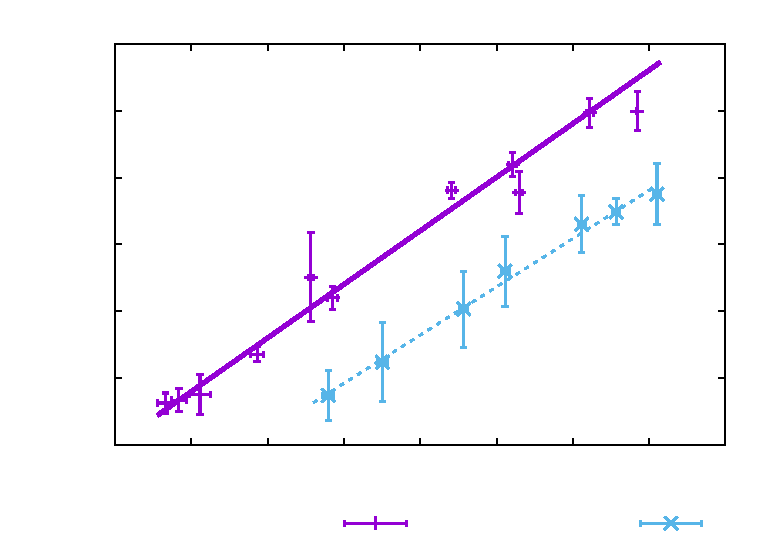
\includegraphics{out_viscos_rat_film_ift}}%
    \gplfronttext
  \end{picture}%
\endgroup
}

      \resizebox{0.9\textwidth}{!}{% GNUPLOT: LaTeX picture with Postscript
\begingroup
  \makeatletter
  \providecommand\color[2][]{%
    \GenericError{(gnuplot) \space\space\space\@spaces}{%
      Package color not loaded in conjunction with
      terminal option `colourtext'%
    }{See the gnuplot documentation for explanation.%
    }{Either use 'blacktext' in gnuplot or load the package
      color.sty in LaTeX.}%
    \renewcommand\color[2][]{}%
  }%
  \providecommand\includegraphics[2][]{%
    \GenericError{(gnuplot) \space\space\space\@spaces}{%
      Package graphicx or graphics not loaded%
    }{See the gnuplot documentation for explanation.%
    }{The gnuplot epslatex terminal needs graphicx.sty or graphics.sty.}%
    \renewcommand\includegraphics[2][]{}%
  }%
  \providecommand\rotatebox[2]{#2}%
  \@ifundefined{ifGPcolor}{%
    \newif\ifGPcolor
    \GPcolortrue
  }{}%
  \@ifundefined{ifGPblacktext}{%
    \newif\ifGPblacktext
    \GPblacktextfalse
  }{}%
  % define a \g@addto@macro without @ in the name:
  \let\gplgaddtomacro\g@addto@macro
  % define empty templates for all commands taking text:
  \gdef\gplbacktext{}%
  \gdef\gplfronttext{}%
  \makeatother
  \ifGPblacktext
    % no textcolor at all
    \def\colorrgb#1{}%
    \def\colorgray#1{}%
  \else
    % gray or color?
    \ifGPcolor
      \def\colorrgb#1{\color[rgb]{#1}}%
      \def\colorgray#1{\color[gray]{#1}}%
      \expandafter\def\csname LTw\endcsname{\color{white}}%
      \expandafter\def\csname LTb\endcsname{\color{black}}%
      \expandafter\def\csname LTa\endcsname{\color{black}}%
      \expandafter\def\csname LT0\endcsname{\color[rgb]{1,0,0}}%
      \expandafter\def\csname LT1\endcsname{\color[rgb]{0,1,0}}%
      \expandafter\def\csname LT2\endcsname{\color[rgb]{0,0,1}}%
      \expandafter\def\csname LT3\endcsname{\color[rgb]{1,0,1}}%
      \expandafter\def\csname LT4\endcsname{\color[rgb]{0,1,1}}%
      \expandafter\def\csname LT5\endcsname{\color[rgb]{1,1,0}}%
      \expandafter\def\csname LT6\endcsname{\color[rgb]{0,0,0}}%
      \expandafter\def\csname LT7\endcsname{\color[rgb]{1,0.3,0}}%
      \expandafter\def\csname LT8\endcsname{\color[rgb]{0.5,0.5,0.5}}%
    \else
      % gray
      \def\colorrgb#1{\color{black}}%
      \def\colorgray#1{\color[gray]{#1}}%
      \expandafter\def\csname LTw\endcsname{\color{white}}%
      \expandafter\def\csname LTb\endcsname{\color{black}}%
      \expandafter\def\csname LTa\endcsname{\color{black}}%
      \expandafter\def\csname LT0\endcsname{\color{black}}%
      \expandafter\def\csname LT1\endcsname{\color{black}}%
      \expandafter\def\csname LT2\endcsname{\color{black}}%
      \expandafter\def\csname LT3\endcsname{\color{black}}%
      \expandafter\def\csname LT4\endcsname{\color{black}}%
      \expandafter\def\csname LT5\endcsname{\color{black}}%
      \expandafter\def\csname LT6\endcsname{\color{black}}%
      \expandafter\def\csname LT7\endcsname{\color{black}}%
      \expandafter\def\csname LT8\endcsname{\color{black}}%
    \fi
  \fi
    \setlength{\unitlength}{0.0500bp}%
    \ifx\gptboxheight\undefined%
      \newlength{\gptboxheight}%
      \newlength{\gptboxwidth}%
      \newsavebox{\gptboxtext}%
    \fi%
    \setlength{\fboxrule}{0.5pt}%
    \setlength{\fboxsep}{1pt}%
\begin{picture}(7200.00,5040.00)%
    \gplgaddtomacro\gplbacktext{%
      \csname LTb\endcsname%
      \put(814,704){\makebox(0,0)[r]{\strut{}$5.5$}}%
      \put(814,1383){\makebox(0,0)[r]{\strut{}$6$}}%
      \put(814,2061){\makebox(0,0)[r]{\strut{}$6.5$}}%
      \put(814,2740){\makebox(0,0)[r]{\strut{}$7$}}%
      \put(814,3418){\makebox(0,0)[r]{\strut{}$7.5$}}%
      \put(814,4097){\makebox(0,0)[r]{\strut{}$8$}}%
      \put(814,4775){\makebox(0,0)[r]{\strut{}$8.5$}}%
      \put(946,484){\makebox(0,0){\strut{}$2.5$}}%
      \put(1678,484){\makebox(0,0){\strut{}$3$}}%
      \put(2410,484){\makebox(0,0){\strut{}$3.5$}}%
      \put(3142,484){\makebox(0,0){\strut{}$4$}}%
      \put(3875,484){\makebox(0,0){\strut{}$4.5$}}%
      \put(4607,484){\makebox(0,0){\strut{}$5$}}%
      \put(5339,484){\makebox(0,0){\strut{}$5.5$}}%
      \put(6071,484){\makebox(0,0){\strut{}$6$}}%
      \put(6803,484){\makebox(0,0){\strut{}$6.5$}}%
      \put(5339,3418){\makebox(0,0){\strut{}4/5}}%
    }%
    \gplgaddtomacro\gplfronttext{%
      \csname LTb\endcsname%
      \put(176,2739){\rotatebox{-270}{\makebox(0,0){\strut{}$\ln(t_{\text{s}} / t_{\text{i}})$}}}%
      \put(3874,154){\makebox(0,0){\strut{}$\ln(\lambda / \Bo)$}}%
    }%
    \gplbacktext
    \put(0,0){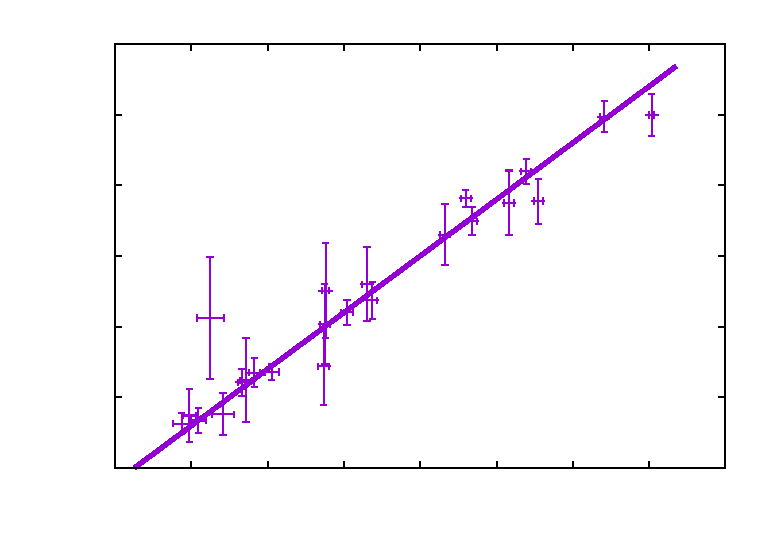
\includegraphics{2D_fit_pretty}}%
    \gplfronttext
  \end{picture}%
\endgroup
}

    \end{column}
  \end{columns}


\end{frame}
%-----------------------------------------------

\begin{frame}
  \frametitle{Sinking Timescales - Tailing}

  \begin{columns}[t]
    \begin{column}{0.5\paperwidth}
      \centering
      \resizebox{\textwidth}{!}{% GNUPLOT: LaTeX picture with Postscript
\begingroup
  \makeatletter
  \providecommand\color[2][]{%
    \GenericError{(gnuplot) \space\space\space\@spaces}{%
      Package color not loaded in conjunction with
      terminal option `colourtext'%
    }{See the gnuplot documentation for explanation.%
    }{Either use 'blacktext' in gnuplot or load the package
      color.sty in LaTeX.}%
    \renewcommand\color[2][]{}%
  }%
  \providecommand\includegraphics[2][]{%
    \GenericError{(gnuplot) \space\space\space\@spaces}{%
      Package graphicx or graphics not loaded%
    }{See the gnuplot documentation for explanation.%
    }{The gnuplot epslatex terminal needs graphicx.sty or graphics.sty.}%
    \renewcommand\includegraphics[2][]{}%
  }%
  \providecommand\rotatebox[2]{#2}%
  \@ifundefined{ifGPcolor}{%
    \newif\ifGPcolor
    \GPcolortrue
  }{}%
  \@ifundefined{ifGPblacktext}{%
    \newif\ifGPblacktext
    \GPblacktextfalse
  }{}%
  % define a \g@addto@macro without @ in the name:
  \let\gplgaddtomacro\g@addto@macro
  % define empty templates for all commands taking text:
  \gdef\gplbacktext{}%
  \gdef\gplfronttext{}%
  \makeatother
  \ifGPblacktext
    % no textcolor at all
    \def\colorrgb#1{}%
    \def\colorgray#1{}%
  \else
    % gray or color?
    \ifGPcolor
      \def\colorrgb#1{\color[rgb]{#1}}%
      \def\colorgray#1{\color[gray]{#1}}%
      \expandafter\def\csname LTw\endcsname{\color{white}}%
      \expandafter\def\csname LTb\endcsname{\color{black}}%
      \expandafter\def\csname LTa\endcsname{\color{black}}%
      \expandafter\def\csname LT0\endcsname{\color[rgb]{1,0,0}}%
      \expandafter\def\csname LT1\endcsname{\color[rgb]{0,1,0}}%
      \expandafter\def\csname LT2\endcsname{\color[rgb]{0,0,1}}%
      \expandafter\def\csname LT3\endcsname{\color[rgb]{1,0,1}}%
      \expandafter\def\csname LT4\endcsname{\color[rgb]{0,1,1}}%
      \expandafter\def\csname LT5\endcsname{\color[rgb]{1,1,0}}%
      \expandafter\def\csname LT6\endcsname{\color[rgb]{0,0,0}}%
      \expandafter\def\csname LT7\endcsname{\color[rgb]{1,0.3,0}}%
      \expandafter\def\csname LT8\endcsname{\color[rgb]{0.5,0.5,0.5}}%
    \else
      % gray
      \def\colorrgb#1{\color{black}}%
      \def\colorgray#1{\color[gray]{#1}}%
      \expandafter\def\csname LTw\endcsname{\color{white}}%
      \expandafter\def\csname LTb\endcsname{\color{black}}%
      \expandafter\def\csname LTa\endcsname{\color{black}}%
      \expandafter\def\csname LT0\endcsname{\color{black}}%
      \expandafter\def\csname LT1\endcsname{\color{black}}%
      \expandafter\def\csname LT2\endcsname{\color{black}}%
      \expandafter\def\csname LT3\endcsname{\color{black}}%
      \expandafter\def\csname LT4\endcsname{\color{black}}%
      \expandafter\def\csname LT5\endcsname{\color{black}}%
      \expandafter\def\csname LT6\endcsname{\color{black}}%
      \expandafter\def\csname LT7\endcsname{\color{black}}%
      \expandafter\def\csname LT8\endcsname{\color{black}}%
    \fi
  \fi
    \setlength{\unitlength}{0.0500bp}%
    \ifx\gptboxheight\undefined%
      \newlength{\gptboxheight}%
      \newlength{\gptboxwidth}%
      \newsavebox{\gptboxtext}%
    \fi%
    \setlength{\fboxrule}{0.5pt}%
    \setlength{\fboxsep}{1pt}%
\begin{picture}(7200.00,5040.00)%
    \gplgaddtomacro\gplbacktext{%
      \csname LTb\endcsname%
      \put(814,1144){\makebox(0,0)[r]{\strut{}$2.5$}}%
      \put(814,1663){\makebox(0,0)[r]{\strut{}$3$}}%
      \put(814,2181){\makebox(0,0)[r]{\strut{}$3.5$}}%
      \put(814,2700){\makebox(0,0)[r]{\strut{}$4$}}%
      \put(814,3219){\makebox(0,0)[r]{\strut{}$4.5$}}%
      \put(814,3738){\makebox(0,0)[r]{\strut{}$5$}}%
      \put(814,4256){\makebox(0,0)[r]{\strut{}$5.5$}}%
      \put(814,4775){\makebox(0,0)[r]{\strut{}$6$}}%
      \put(946,924){\makebox(0,0){\strut{}$-0.2$}}%
      \put(1597,924){\makebox(0,0){\strut{}$0$}}%
      \put(2248,924){\makebox(0,0){\strut{}$0.2$}}%
      \put(2898,924){\makebox(0,0){\strut{}$0.4$}}%
      \put(3549,924){\makebox(0,0){\strut{}$0.6$}}%
      \put(4200,924){\makebox(0,0){\strut{}$0.8$}}%
      \put(4851,924){\makebox(0,0){\strut{}$1$}}%
      \put(5501,924){\makebox(0,0){\strut{}$1.2$}}%
      \put(6152,924){\makebox(0,0){\strut{}$1.4$}}%
      \put(6803,924){\makebox(0,0){\strut{}$1.6$}}%
      \put(3549,2596){\makebox(0,0){\strut{}\normalsize $-1.6 \pm 0.3$}}%
      \put(5501,2700){\makebox(0,0){\strut{}\normalsize $-1.5 \pm 0.2$}}%
      \put(2898,4256){\makebox(0,0){\strut{}\normalsize $-0.92 \pm 0.06$}}%
      \put(5176,3997){\makebox(0,0){\strut{}\normalsize $0.06 \pm 0.01$}}%
    }%
    \gplgaddtomacro\gplfronttext{%
      \csname LTb\endcsname%
      \put(176,2959){\rotatebox{-270}{\makebox(0,0){\strut{}$\ln(t / t_{i})$}}}%
      \put(3874,594){\makebox(0,0){\strut{}$\ln\text{Bo}$}}%
      \csname LTb\endcsname%
      \put(3019,393){\makebox(0,0)[r]{\strut{}$1 < \lambda < 3$}}%
      \csname LTb\endcsname%
      \put(3019,173){\makebox(0,0)[r]{\strut{}$3 < \lambda < 6$}}%
      \csname LTb\endcsname%
      \put(5854,393){\makebox(0,0)[r]{\strut{}$7 < \lambda < \; \, 9$}}%
      \csname LTb\endcsname%
      \put(5854,173){\makebox(0,0)[r]{\strut{}$17 < \lambda < 20$}}%
    }%
    \gplbacktext
    \put(0,0){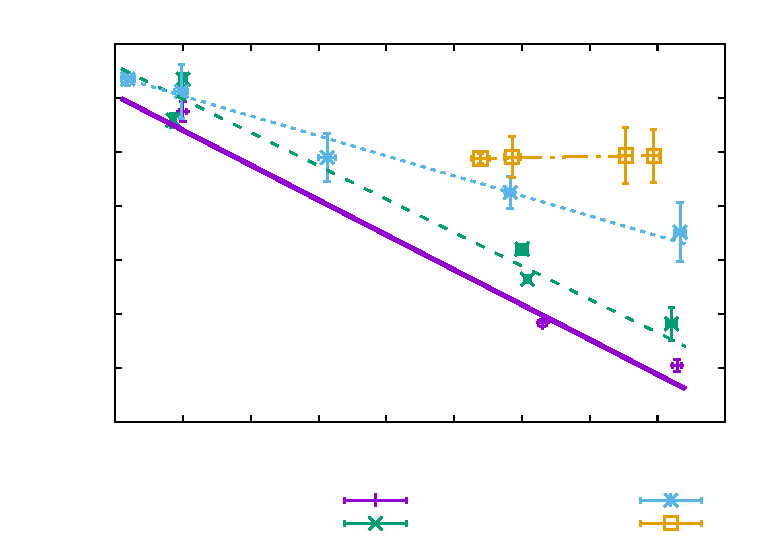
\includegraphics{out_bond_tail}}%
    \gplfronttext
  \end{picture}%
\endgroup
}

      A power law dependence on Bond number \\
      \vspace{0.5cm}
      But exponenent depends on viscosity ratio \\
      
    \end{column}

    \begin{column}{0.5\paperwidth}
      \centering
      \resizebox{\textwidth}{!}{% GNUPLOT: LaTeX picture with Postscript
\begingroup
  \makeatletter
  \providecommand\color[2][]{%
    \GenericError{(gnuplot) \space\space\space\@spaces}{%
      Package color not loaded in conjunction with
      terminal option `colourtext'%
    }{See the gnuplot documentation for explanation.%
    }{Either use 'blacktext' in gnuplot or load the package
      color.sty in LaTeX.}%
    \renewcommand\color[2][]{}%
  }%
  \providecommand\includegraphics[2][]{%
    \GenericError{(gnuplot) \space\space\space\@spaces}{%
      Package graphicx or graphics not loaded%
    }{See the gnuplot documentation for explanation.%
    }{The gnuplot epslatex terminal needs graphicx.sty or graphics.sty.}%
    \renewcommand\includegraphics[2][]{}%
  }%
  \providecommand\rotatebox[2]{#2}%
  \@ifundefined{ifGPcolor}{%
    \newif\ifGPcolor
    \GPcolortrue
  }{}%
  \@ifundefined{ifGPblacktext}{%
    \newif\ifGPblacktext
    \GPblacktextfalse
  }{}%
  % define a \g@addto@macro without @ in the name:
  \let\gplgaddtomacro\g@addto@macro
  % define empty templates for all commands taking text:
  \gdef\gplbacktext{}%
  \gdef\gplfronttext{}%
  \makeatother
  \ifGPblacktext
    % no textcolor at all
    \def\colorrgb#1{}%
    \def\colorgray#1{}%
  \else
    % gray or color?
    \ifGPcolor
      \def\colorrgb#1{\color[rgb]{#1}}%
      \def\colorgray#1{\color[gray]{#1}}%
      \expandafter\def\csname LTw\endcsname{\color{white}}%
      \expandafter\def\csname LTb\endcsname{\color{black}}%
      \expandafter\def\csname LTa\endcsname{\color{black}}%
      \expandafter\def\csname LT0\endcsname{\color[rgb]{1,0,0}}%
      \expandafter\def\csname LT1\endcsname{\color[rgb]{0,1,0}}%
      \expandafter\def\csname LT2\endcsname{\color[rgb]{0,0,1}}%
      \expandafter\def\csname LT3\endcsname{\color[rgb]{1,0,1}}%
      \expandafter\def\csname LT4\endcsname{\color[rgb]{0,1,1}}%
      \expandafter\def\csname LT5\endcsname{\color[rgb]{1,1,0}}%
      \expandafter\def\csname LT6\endcsname{\color[rgb]{0,0,0}}%
      \expandafter\def\csname LT7\endcsname{\color[rgb]{1,0.3,0}}%
      \expandafter\def\csname LT8\endcsname{\color[rgb]{0.5,0.5,0.5}}%
    \else
      % gray
      \def\colorrgb#1{\color{black}}%
      \def\colorgray#1{\color[gray]{#1}}%
      \expandafter\def\csname LTw\endcsname{\color{white}}%
      \expandafter\def\csname LTb\endcsname{\color{black}}%
      \expandafter\def\csname LTa\endcsname{\color{black}}%
      \expandafter\def\csname LT0\endcsname{\color{black}}%
      \expandafter\def\csname LT1\endcsname{\color{black}}%
      \expandafter\def\csname LT2\endcsname{\color{black}}%
      \expandafter\def\csname LT3\endcsname{\color{black}}%
      \expandafter\def\csname LT4\endcsname{\color{black}}%
      \expandafter\def\csname LT5\endcsname{\color{black}}%
      \expandafter\def\csname LT6\endcsname{\color{black}}%
      \expandafter\def\csname LT7\endcsname{\color{black}}%
      \expandafter\def\csname LT8\endcsname{\color{black}}%
    \fi
  \fi
    \setlength{\unitlength}{0.0500bp}%
    \ifx\gptboxheight\undefined%
      \newlength{\gptboxheight}%
      \newlength{\gptboxwidth}%
      \newsavebox{\gptboxtext}%
    \fi%
    \setlength{\fboxrule}{0.5pt}%
    \setlength{\fboxsep}{1pt}%
\begin{picture}(7200.00,5040.00)%
    \gplgaddtomacro\gplbacktext{%
      \csname LTb\endcsname%
      \put(814,1144){\makebox(0,0)[r]{\strut{}$2.5$}}%
      \put(814,1663){\makebox(0,0)[r]{\strut{}$3$}}%
      \put(814,2181){\makebox(0,0)[r]{\strut{}$3.5$}}%
      \put(814,2700){\makebox(0,0)[r]{\strut{}$4$}}%
      \put(814,3219){\makebox(0,0)[r]{\strut{}$4.5$}}%
      \put(814,3738){\makebox(0,0)[r]{\strut{}$5$}}%
      \put(814,4256){\makebox(0,0)[r]{\strut{}$5.5$}}%
      \put(814,4775){\makebox(0,0)[r]{\strut{}$6$}}%
      \put(946,924){\makebox(0,0){\strut{}$-2$}}%
      \put(1922,924){\makebox(0,0){\strut{}$-1$}}%
      \put(2898,924){\makebox(0,0){\strut{}$0$}}%
      \put(3875,924){\makebox(0,0){\strut{}$1$}}%
      \put(4851,924){\makebox(0,0){\strut{}$2$}}%
      \put(5827,924){\makebox(0,0){\strut{}$3$}}%
      \put(6803,924){\makebox(0,0){\strut{}$4$}}%
    }%
    \gplgaddtomacro\gplfronttext{%
      \csname LTb\endcsname%
      \put(176,2959){\rotatebox{-270}{\makebox(0,0){\strut{}$\ln(t / t_{i})$}}}%
      \put(3874,594){\makebox(0,0){\strut{}$\ln \lambda$}}%
      \csname LTb\endcsname%
      \put(3019,393){\makebox(0,0)[r]{\strut{}$0.75 < \text{Bo} < 1.25$}}%
      \csname LTb\endcsname%
      \put(3019,173){\makebox(0,0)[r]{\strut{}$1.25 < \text{Bo} < 1.75$}}%
      \csname LTb\endcsname%
      \put(6250,393){\makebox(0,0)[r]{\strut{}$2 < \text{Bo} < \; \; \: 3$}}%
      \csname LTb\endcsname%
      \put(6250,173){\makebox(0,0)[r]{\strut{}$3.5 < \text{Bo} < 4.5$}}%
    }%
    \gplbacktext
    \put(0,0){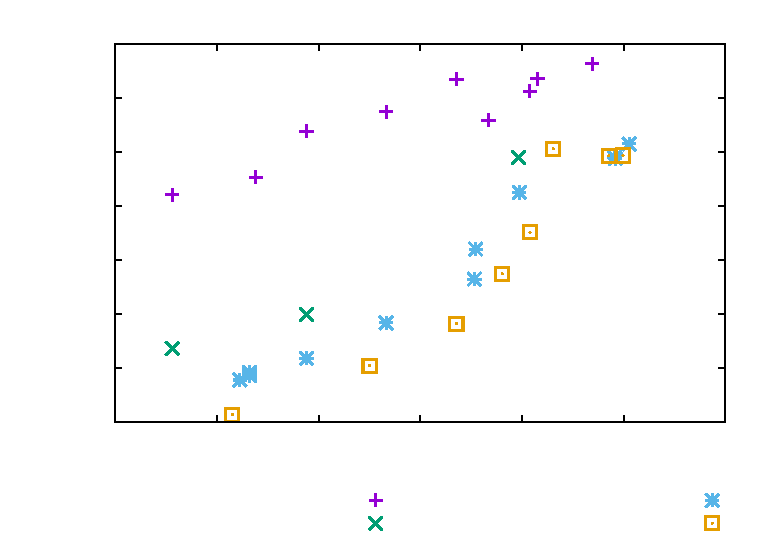
\includegraphics{out_viscos_rat_tail_ift}}%
    \gplfronttext
  \end{picture}%
\endgroup
}
      
      \vspace{1cm}
      $\frac{t}{t_{\text{i}}} \sim \Bo^{a(\lambda)} \lambda^{b}$

      \vspace{1cm}

      Clearly need more data
    \end{column}
  \end{columns}


\end{frame}
%-----------------------------------------------


\begin{frame}
  \frametitle{Hypothesis - Two stage sinking}

  \vspace{-0.5cm}

  \begin{columns}[t]

    \begin{column}{0.5\paperwidth}

      \centering

      Tail formation stretching and thinning

      \vspace{-0.5cm}

      \begin{figure}
        $$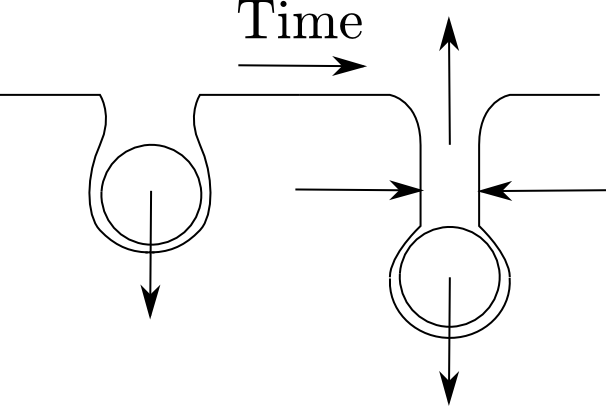
\includegraphics[width=0.9\textwidth]{tail_thinning.png}$$
      \end{figure}

      \vspace{-0.5cm}

      Tail thickness $> l_{\text{c}}$

    \end{column}

    \begin{column}{0.5\paperwidth}

      \centering

      Tail Rupture

      \vspace{-0.5cm}

      \begin{figure}
        $$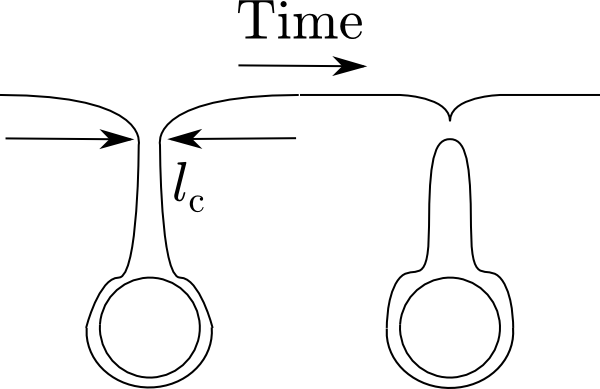
\includegraphics[width=0.9\textwidth]{tail_rupture.png}$$
      \end{figure}

      \vspace{-0.5cm}

      Tail thickness $\sim l_{\text{c}}$

    \end{column}

  \end{columns}

  \vspace{0.5cm}

  Each stage is associated with it's own timescale

  When $Bo \lesssim 1$, $a \lesssim l_{\text{c}}$, sinking timescale dominated by rupture stage
\end{frame}
%-----------------------------------------------

\begin{frame}
  \frametitle{Summary}

  Studied Low Reynolds number settling of spheres through interface between density-stratified, immiscible fluids \\

  \vspace{0.75cm}

  When does entrainment occur?
  \begin{itemize}
  \item For $\text{Bo} > 1$ and $\lambda < 30$ passage of sphere entrains fluid from upper phase \\
  \item As $\text{Bo}$ decreases, value of $\lambda$ at which transition occurs decreases \\
  \end{itemize}

  \vspace{0.75cm}

  What is the timescale of sinking?
  \begin{itemize}
  \item For film drainage $t / t_{\text{i}} \sim (\lambda / \text{Bo})^{4/5}$ \\
  \item Tailing mode - power law dependence on $\text{Bo}$ but exponent depends on $\lambda$ ? \\
  \item More data needed, but hypothesise two-stage sinking process \\
  \end{itemize}

\end{frame}
%-----------------------------------------------

\end{document}